%% ============================================================
%% Appendix (included after \appendix in main.tex)
%% ============================================================

%% ============================================================
\section{Complete Formalization of CRAFT}
\label{app:formal-method}
%% ============================================================

This section expands the method in Section~\ref{sec:method} into a complete
input-to-output specification.  Given a task with hidden goals, CRAFT masks
those goals and applies the same rollout--decompose--pool--filter--compose
operator at inference time and during label construction.  We first define
the program semantics and verifier, then the exact and resource-bounded
filters, and finally the inference, SFT, and RL procedures.  Shapley credit and group reward collapse are formalized alongside RL scoring
and policy updates; the remaining theoretical properties and proofs are
collected in Appendix~\ref{app:composition-proofs} within this formalization.

\subsection{Task Semantics, Loop Invariants, and Verification}
\label{app:formal-loop-verification}

Let \(\Sigma\) be the program-state space.  A loop is
\(\mathcal L=(\mathsf{Init},B,S)\), where \(\mathsf{Init}\) characterizes the
first loop-head states, \(B\) is the guard, and
\(S\subseteq\Sigma\times\Sigma\) is one normally completing loop step.  Thus
\(S(\sigma,\sigma')\) includes execution of the body and any guard or update
side effects required to reach the next loop head.

\begin{definition}[Inductive invariant]
\label{def:formal-inductive}
A predicate \(I\) is a valid loop invariant when
\begin{equation}
  \begin{split}
  &\forall\sigma\in\Sigma:\
    \mathsf{Init}(\sigma)\Rightarrow I(\sigma),\\
  &\forall\sigma,\sigma'\in\Sigma:\
    I(\sigma)\land B(\sigma)\land S(\sigma,\sigma')
    \Rightarrow I(\sigma').
  \end{split}
  \label{eq:formal-inductive}
\end{equation}
We denote these two obligations by \(\operatorname{Ind}_{\mathcal L}(I)\).
Here and throughout the paper, \emph{valid invariant} means inductive in this
sense.  This implies validity on every reachable loop-head state, although the
converse need not hold for the chosen assertion language and prover.
\end{definition}

A response is decomposed into a finite candidate family \(C\) of clauses.  The
clauses compose by conjunction,
\begin{equation}
  I(C)=\bigwedge_{c\in C}c,
  \qquad I(\varnothing)=\mathit{true}.
  \label{eq:formal-compose}
\end{equation}
The set \(C\) is \emph{jointly inductive} when
\(\operatorname{Ind}_{\mathcal L}(I(C))\) holds.  Notice that preservation is
checked under the full conjunction: a clause may rely on companion clauses.
The logical definition is insensitive to clause order.  The bounded verifier,
however, receives a deterministic sequence
\(D=\langle d_1,\ldots,d_m\rangle\), because generated proof dependencies can
follow annotation order.  Set notation below denotes the members of this
sequence; deletion preserves their relative order.

A complete task is \(\mathcal T=(\mathcal L,\mathcal G)\), where
\(\mathcal G\) contains the assertions and postconditions at their original
program locations.  For a body target, let
\(S^{B}_{\ell}\subseteq\Sigma\times\Sigma\) be the path-sensitive prefix
relation from the loop head through guard evaluation to \(\ell\).
For a target after the loop, let \(E_0\) be the guard-false exit relation
and \(E_b\) the relation from a loop head through the body prefix to a
\texttt{break} that exits this loop.  These relations include guard and
branch conditions and all side effects.  Let \(F_{e,\ell}\) be the suffix
from exit \(e\) to \(\ell\), the identity for an immediately following
target.  Define the complete exit-to-target relation by
\[
 X_\ell(\sigma,\sigma')\iff
 \bigvee_{e\in\{0\}\cup\mathcal B}
 \exists\eta:\ E_e(\sigma,\eta)\land F_{e,\ell}(\eta,\sigma'),
\]
where \(\mathcal B\) indexes the loop's break exits.  For a side-effect-free
guard, \(E_0(\sigma,\eta)\) is \(\neg B(\sigma)\land\eta=\sigma\).
Unlike \(E_0\), a break exit may start with \(B(\sigma)\) true.
Then define
\begin{equation}
  \operatorname{VC}_{\mathcal L}(I,\ell,g)=
  \begin{cases}
    \forall\sigma,\sigma':
    I(\sigma)\land S^{B}_{\ell}(\sigma,\sigma')
    \Rightarrow g(\sigma'),
      & \ell\text{ is inside the body},\\
    \forall\sigma,\sigma':
    I(\sigma)\land X_\ell(\sigma,\sigma')
    \Rightarrow g(\sigma'),
      & \ell\text{ is after the loop}.
  \end{cases}
  \label{eq:formal-target-vc}
\end{equation}
Postconditions are represented by the second case, with suffix relations
including assignments and return-value substitution.  A return or other
abrupt exit inside the body, when admitted, requires its own exit relation
and applicable target obligations in the same union; it does not contribute
to the normally completing transition \(S\).  For example, with
\texttt{while (1) \{ if (q) break; ... \}}, the guard-false branch is empty,
but the break branch still yields a nonvacuous post-loop obligation.
The ideal logical verdict is
\begin{equation}
  \operatorname{TaskValid}_{\models}(\mathcal T,C)
  =\operatorname{Ind}_{\mathcal L}(I(C))\land
   \bigwedge_{(\ell,g)\in\mathcal G}
   \operatorname{VC}_{\mathcal L}(I(C),\ell,g).
  \label{eq:formal-verify}
\end{equation}
Generation and training see only \(\mathcal L\); \(\mathcal G\) is restored
only for Equation~\eqref{eq:formal-verify}.

For a proof goal \(g\) generated by the configured loop verifier, define its
portfolio status by
\begin{equation}
  \operatorname{GoalStatus}_{\delta}(g)
  \in\{\mathsf{valid},\mathsf{timeout},\mathsf{unknown}\},
  \label{eq:formal-goal-status}
\end{equation}
where \(\mathsf{valid}\) means that at least one configured prover returned
\emph{Valid}; \(\mathsf{timeout}\) means that no prover proved the goal and at
least one exhausted \(\delta\); and \(\mathsf{unknown}\) contains every other
non-valid, unsupported, missing, or malformed result.

Let \(\mathcal S_{\mathrm{ver}}=
\{\mathsf{valid},\mathsf{timeout},\mathsf{unknown}\}\).  One invocation
of the resource-bounded loop verifier on the current ordered family
\(D=\langle d_1,\ldots,d_m\rangle\) returns the clause-to-status map
\begin{equation}
  \operatorname{LoopVerify}_{\mathcal L,\delta}(D)
  =\{d_k\mapsto v_{D,k}:1\le k\le m\}
  \in\mathcal S_{\mathrm{ver}}^{D},
  \label{eq:formal-loop-verify-map}
\end{equation}
where \(v_{D,k}=\mathsf{valid}\) means that the verifier proves all
establishment and preservation obligations generated for \(d_k\) in the
current family \(D\).  If the obligations are not all proved,
\(v_{D,k}=\mathsf{timeout}\) records an exhausted prover budget and
\(v_{D,k}=\mathsf{unknown}\) records every other outcome.  The interface is
sound when
\begin{equation}
  \left(\forall c\in D:\
    \operatorname{LoopVerify}_{\mathcal L,\delta}(D)[c]=\mathsf{valid}\right)
  \Longrightarrow \operatorname{Ind}_{\mathcal L}(I(D)).
  \label{eq:formal-loop-verify-soundness}
\end{equation}
The filter treats \(\mathsf{timeout}\) and \(\mathsf{unknown}\) identically,
but the interface keeps them distinct.  Appendix~\ref{app:loop-verifier-realization}
describes how the implementation generates and aggregates the clause goals.

After the invariant set is fixed, the separate binary operator
\(\operatorname{TaskVerify}_{\delta}(\mathcal T,C)\) runs the verifier on the
original task annotated with \(C\).  Let
\(\operatorname{TargetGoals}(\mathcal T,C)\) be its generated source-level
assertion and postcondition goals.  Then
\begin{equation}
\begin{split}
\operatorname{TaskVerify}_{\delta}(\mathcal T,C)
=\mathbf 1\bigl[&\operatorname{SyntaxOK}(\mathcal T,C)\ \land\\
&\forall c\in C:\
  \operatorname{LoopVerify}_{\mathcal L,\delta}(C)[c]=\mathsf{valid}\ \land\\
&\forall g\in\operatorname{TargetGoals}(\mathcal T,C):
  \operatorname{GoalStatus}_{\delta}(g)=\mathsf{valid}\bigr].
\end{split}
\label{eq:formal-task-verify}
\end{equation}

\subsection{Ideal and Resource-Bounded Houdini Filtering}
\label{app:formal-houdini}

We define an exact semantic fixed-point operator and its resource-bounded
verifier counterpart.

For \(c\in C\), define its establishment and context-dependent preservation
obligations by
\begin{equation}
  \begin{split}
  \operatorname{Est}_{\mathcal L}(c)
    &\iff \forall\sigma:\
      \mathsf{Init}(\sigma)\Rightarrow c(\sigma),\\
  \operatorname{Pres}_{\mathcal L,C}(c)
    &\iff \forall\sigma,\sigma':
      I(C)(\sigma)\land B(\sigma)\land S(\sigma,\sigma')
      \Rightarrow c(\sigma').
  \end{split}
  \label{eq:formal-clause-obligations}
\end{equation}
Ideal Houdini starts with \(C_0=C\) and repeats
\begin{equation}
  C_{j+1}=\mathsf F_{\mathcal L}(C_j)
  =\{c\in C_j:\operatorname{Est}_{\mathcal L}(c)
    \land\operatorname{Pres}_{\mathcal L,C_j}(c)\}
  \label{eq:formal-houdini}
\end{equation}
until a fixed point \(\mathsf H_{\mathcal L}(C)\) is reached.

The implemented deletion round uses the clause-level loop verifier and
preserves the relative order of retained clauses:
\begin{equation}
  \widehat{\mathsf F}_{\mathcal L,\delta}(D)
  =\left\langle c\in D\ \middle|\
    \operatorname{LoopVerify}_{\mathcal L,\delta}(D)[c]=\mathsf{valid}
  \right\rangle.
  \label{eq:formal-bounded-houdini-round}
\end{equation}
Thus timeout and unknown both cause conservative deletion.  Every status in
one round is computed under the same pre-deletion context \(D\).  A clause
removed at the end of that round may therefore have helped another clause
receive \(\mathsf{valid}\).  The survivors must be verified again without the
removed hypotheses; this is why a single deletion pass is insufficient.  For
an ordered input sequence \(D\), let \(D_0=D\) and
\(D_{j+1}=\widehat{\mathsf F}_{\mathcal L,\delta}(D_j)\).  Iteration stops at
the first proved fixed point or at the symbolic round limit \(h_{\max}\).  Let
\begin{equation}
  j^*=\min\{j<h_{\max}:
    \widehat{\mathsf F}_{\mathcal L,\delta}(D_j)=D_j\},
  \label{eq:formal-bounded-fixed-point}
\end{equation}
when this set is nonempty.  The implemented filter is
\begin{equation}
  \operatorname{Filter}_{\mathcal L}^{\delta,h_{\max}}(D)=
  \begin{cases}
    D_{j^*}, & j^*\text{ exists},\\
    \langle\rangle, & \text{the round limit is reached first}.
  \end{cases}
  \label{eq:formal-bounded-houdini}
\end{equation}
At a returned fixed point, every surviving clause has just been proved in the
context of that same sequence.  Reaching the limit returns the empty sequence.  Under a
sound loop verifier, the result is sound and may be smaller than the ideal
fixed point.  In
the remainder, \(\operatorname{Filter}_{\mathcal L}\) abbreviates
Equation~\eqref{eq:formal-bounded-houdini}, and
\(\operatorname{TaskVerify}\) abbreviates
\(\operatorname{TaskVerify}_{\delta}\).

\subsection{The Shared Composition Operator}

Let \(\operatorname{parts}(y)\) extract the ordered sequence of invariant
clauses in response \(y\), let \(\operatorname{First}_{m}(L)\) be the prefix
of sequence \(L\) containing at most \(m\) clauses, and let \(\Vert\) denote
sequence concatenation.  Define the clauses admitted from one response by
\begin{equation}
  \operatorname{Admit}(y)=
  \operatorname{Unique}\!\left(
    \operatorname{First}_{m_{\max}}(\operatorname{parts}(y))
  \right).
  \label{eq:formal-admit}
\end{equation}
\(\operatorname{Unique}\) removes duplicates using the finite-rule
canonical normalization \(\operatorname{key}(c)\).  Equal keys identify the
clauses merged by those rules.  Provenance is retained by
recording which responses supplied each key.  It keeps the first occurrence;
concatenations are traversed in response order and then clause order, which
fixes the sequence supplied to \(\operatorname{LoopVerify}\).
For a clause sequence \(D\), let
\(\operatorname{keys}(D)=\langle\operatorname{key}(c):c\in D\rangle\).

For any response sequence \(y_{1:n}\), define
\begin{align}
  A_i&=\operatorname{Admit}(y_i),
  &P(y_{1:n})&=\operatorname{Unique}\!\left(A_1\Vert\cdots\Vert A_n\right),
  \label{eq:formal-pool}\\
  C(y_{1:n})&=\operatorname{Filter}_{\mathcal L}(P(y_{1:n})),
  &I(y_{1:n})&=\bigwedge_{c\in C(y_{1:n})}c.
  \label{eq:formal-craft-map}
\end{align}
This is the shared rollout--decompose--pool--filter--compose operator.  The
filter checks preservation under the complete current conjunction, so clauses
from different responses may support one another; standalone preservation is
not required.

\subsection{Complete Inference Algorithm}

\begin{algorithm}[H]
\caption{CRAFT inference}
\label{alg:rcf}
\begin{algorithmic}
\alginput{task \(\mathcal T=(\mathcal L,\mathcal G)\), policy \(\pi\), number of responses \(n\)}
\algoutput{composed invariant \(I\), final verdict \(v\)}
\algline \(x\leftarrow\operatorname{Mask}(\mathcal T)=\mathcal L\)\cmnt{hide goals}\\
\algline sample \(y_{1:n}\sim\pi(\cdot\mid x)\)\cmnt{rollout}\\
\algline \(A_i\leftarrow\operatorname{Admit}(y_i)\) for every \(i\)\cmnt{decompose and cap}\\
\algline \(P\leftarrow\operatorname{Unique}(A_1\Vert\cdots\Vert A_n)\)\cmnt{pool}\\
\algline \(C\leftarrow\operatorname{Filter}_{\mathcal L}^{\delta,h_{\max}}(P)\)\cmnt{filter}\\
\algline \(I\leftarrow\bigwedge_{c\in C}c\)\cmnt{compose}\\
\algline \(v\leftarrow\operatorname{TaskVerify}_{\delta}(\mathcal T,C)\)\cmnt{restore goals}\\
\algline \kw{return} \((I,v)\)\\
\end{algorithmic}
\end{algorithm}

For evaluation, compose@\(n\) is the percentage of tasks for which
\(\operatorname{TaskVerify}(\mathcal T,C(y_{1:n}))\) succeeds on the first
\(n\) saved responses. Pass@\(n\) is the percentage of tasks for which
at least one of these same \(n\) responses independently verifies the targets
(Appendix~\ref{app:experimental-protocol}).

\subsection{Complete SFT Label Construction}

SFT distills the same multi-response map into one response.  It accumulates
raw candidates so that a clause discarded in one round can later acquire a
supporting companion.  The policy \(\pi_0\) is the small open-weight model
being trained and is the only learned generator in label construction.
Executions of \(\mathcal L\) produce the trace signal, and
\(\operatorname{Filter}_{\mathcal L}\) supplies the verifier decision; no
external model supplies candidates, labels, or acceptance judgments.

\begin{algorithm}[H]
\caption{Multi-response SFT synthesis}
\label{alg:formal-sft}
\begin{algorithmic}
\alginput{masked loop \(\mathcal L\), policy \(\pi_0\), negatives \(\mathcal N\), group size \(g_{\mathrm{sft}}\), round limit \(t_{\mathrm{sft}}\)}
\algoutput{one serialized label, or \(\mathsf{reject}\)}
\algline \kw{if} \(\mathcal N=\varnothing\) \kw{then return} \(\mathsf{reject}\)\\
\algline \(P\leftarrow\langle\rangle\)\\
\algline \kw{for} \(t=1,\ldots,t_{\mathrm{sft}}\) \kw{do}\\
\algline \algind sample a response group \(y_{1:g_{\mathrm{sft}}}\sim\pi_0(\cdot\mid\mathcal L)\)\\
\algline \algind \(P\leftarrow\operatorname{Unique}(P\Vert
  \operatorname{Admit}(y_1)\Vert\cdots\Vert
  \operatorname{Admit}(y_{g_{\mathrm{sft}}}))\)\\
\algline \algind \(C\leftarrow\operatorname{Filter}_{\mathcal L}(P)\)\\
\algline \algind \kw{if} \(\operatorname{cov}_{\mathcal N}(C)\ge\tau\)
  \kw{then return} \(\operatorname{Serialize}(C)\)\\
\algline \kw{return} \(\mathsf{reject}\)\\
\end{algorithmic}
\end{algorithm}

The SFT input and label contain no element of \(\mathcal G\).  The parameter
values appear in Appendix~\ref{app:constants}.

\subsection{Complete RL Group-Scoring Algorithm}

The sampled policy is the same small open-weight model updated by RL.  Given
its rollouts, every reward component below is computed from program
executions, verifier outcomes, and deterministic clause provenance; no
external model enters the scoring function.

Executions of the masked loop yield reachable loop-head states \(\mathcal E\)
and target-independent negative traces \(\mathcal N\).  The lightweight
evaluator is three-valued:
\begin{equation}
  \operatorname{Eval}(c,s)\in
  \{\mathsf{true},\mathsf{false},\mathsf{unknown}\}.
  \label{eq:formal-state-eval}
\end{equation}
An unknown result leaves the negative trace unrejected and the candidate out
of the reachable-state front end's accepted set; the verifier handles syntax
and induction.
A trace counts as rejected only when at least one retained clause evaluates
definitively to false at one of its states:
\begin{equation}
  \operatorname{rej}_{\mathcal N}(C)
  =\{\nu\in\mathcal N:\exists s\in\nu,\exists c\in C,\
    \operatorname{Eval}(c,s)=\mathsf{false}\},
  \qquad
  \operatorname{cov}_{\mathcal N}(C)
  =\frac{|\operatorname{rej}_{\mathcal N}(C)|}{|\mathcal N|}.
  \label{eq:formal-coverage}
\end{equation}
Coverage is trajectory level and is defined only for
\(|\mathcal N|>0\).  Instances without retained negatives are rejected during
SFT construction.  For RL, the explicit fallback below uses a binary survivor
signal and never evaluates this ratio.

For an RL group \(y_{1:g_{\mathrm{rl}}}\), first form the same globally
deduplicated pool used at inference, and then invoke the verifier filter once:
\begin{align}
  A_i&=\operatorname{Admit}(y_i),
  &P^*&=\operatorname{Unique}\!\left(A_1\Vert\cdots\Vert A_{g_{\mathrm{rl}}}\right),
  \label{eq:formal-pooled-filter}\\
  C^*&=\operatorname{Filter}_{\mathcal L}(P^*),
  &V_i&=\left\langle c\in A_i\ \middle|\
    \operatorname{key}(c)\in\operatorname{keys}(C^*)\right\rangle,
  &R_i&=\operatorname{rej}_{\mathcal N}(V_i).
  \label{eq:formal-projection}
\end{align}
Here \(V_i\) assigns each pooled survivor back to every response that proposed
it.  A reachable-state front end evaluates the globally pooled candidates on
\(\mathcal E\) before the verifier processes the same pool.  If
\(f(\nu)=|\{j:\nu\in R_j\}|\), the reward is
\begin{equation}
  r_i=w_c\frac{|R_i|}{|\mathcal N|}
      +w_g\left(
        \frac{1}{|\mathcal N|}\sum_{\nu\in R_i}\frac{1}{f(\nu)}
      \right).
  \label{eq:formal-reward}
\end{equation}
Here \(w_c=1.0\) and \(w_g=0.3\) weight coverage and group credit.  The first term rewards each response by the negative coverage of
its pooled survivors.  The second is the response-level Shapley value of the
fixed post-filter coverage game
\(u(A)=|\bigcup_{i\in A}R_i|/|\mathcal N|\): repeated coverage is shared among
its proposers, while unique coverage receives full credit.  Thus
\(1/f(\nu)\) is a group-local difficulty weight: negatives rejected by many
responses receive less credit per response than rare negatives rejected by
few.  The negatives are nonuniformly weighted for each response, while their
credits still sum to one unit per covered trace across the group.
The per-response cap limits admission without penalizing
excess output.

\begin{algorithm}[H]
\caption{CRAFT reward for one RL group}
\label{alg:formal-rl-reward}
\begin{algorithmic}
\alginput{masked loop \(\mathcal L\), responses \(y_{1:g_{\mathrm{rl}}}\), reachable states \(\mathcal E\), negative traces \(\mathcal N\)}
\algoutput{response rewards \(r_{1:g_{\mathrm{rl}}}\)}
\algline \(A_i\leftarrow\operatorname{Admit}(y_i)\) for every \(i\)\\
\algline \(P^*\leftarrow\operatorname{Unique}(A_1\Vert\cdots\Vert
  A_{g_{\mathrm{rl}}})\)\cmnt{pool globally}\\
\algline \(C^*\leftarrow\operatorname{Filter}_{\mathcal L}(P^*)\)
  \cmnt{filter the pool once}\\
\algline \(V_i\leftarrow\langle c\in A_i\mid\operatorname{key}(c)\in
  \operatorname{keys}(C^*)\rangle\) for every \(i\)\cmnt{project by provenance}\\
\algline \kw{if} \(\mathcal N=\varnothing\) \kw{then}\\
\algline \algind \(r_i\leftarrow\mathbf 1[A_i\ne\langle\rangle\ \land\
  \operatorname{keys}(V_i)=\operatorname{keys}(A_i)]\) for every \(i\)\\
\algline \algind \kw{return} \(r_{1:g_{\mathrm{rl}}}\)\\
\algline \(R_i\leftarrow\operatorname{rej}_{\mathcal N}(V_i)\) for every \(i\)\\
\algline \(f(\nu)\leftarrow|\{j:\nu\in R_j\}|\) for every \(\nu\in\mathcal N\)\\
\algline \(r_i\leftarrow w_c|R_i|/|\mathcal N|+
  w_g|\mathcal N|^{-1}\sum_{\nu\in R_i}f(\nu)^{-1}\)
  for every \(i\)\\
\algline \kw{return} \(r_{1:g_{\mathrm{rl}}}\)\\
\end{algorithmic}
\end{algorithm}

A clause \(c\) \emph{semantically supports} \(d\) in \(D\) when
\(c\ne d\), \(\operatorname{Pres}_{\mathcal L,D}(d)\) holds, but
\(\operatorname{Pres}_{\mathcal L,D\setminus\{c\}}(d)\) does not.  The
implemented verifier exposes the broader, resource-dependent relation
\begin{equation}
\begin{split}
\operatorname{VSupport}_{\mathcal L,\delta}(c,d\mid D)
\iff{}&c\ne d\ \land
\operatorname{LoopVerify}_{\mathcal L,\delta}(D)[d]=\mathsf{valid}\ \land\\
&\operatorname{LoopVerify}_{\mathcal L,\delta}(D\setminus\{c\})[d]
  \ne\mathsf{valid}.
\end{split}
\label{eq:formal-verifier-support}
\end{equation}
This relation includes semantic support, generated-goal dependencies, and
resource effects.  Algorithm~\ref{alg:formal-rl-reward} can retain such a
clause through joint filtering.

\subsubsection{Shapley Credit: Definition and Equivalence}
\label{app:formal-shapley}

Fix the survivor bundles from one pooled filtering call and write
\(R_i=\operatorname{rej}_{\mathcal N}(V_i)\) and
\(f(\nu)=|\{j:\nu\in R_j\}|\).  For nonempty \(\mathcal N\),
\begin{equation}
  \begin{aligned}
  r_i^{\text{Clause-decomposed}}&=\frac{|R_i|}{|\mathcal N|},
  &\phi_i&=\frac{1}{|\mathcal N|}\sum_{\nu\in R_i}\frac{1}{f(\nu)},\\
  r_i^{\mathrm{Full}}&=r_i^{\text{Clause-decomposed}}+0.3\phi_i.
  \end{aligned}
  \label{eq:shapley-credit}
\end{equation}
\paragraph{Equivalence to the standard Shapley value.}
Equation~\eqref{eq:shapley-credit} gives a closed form for the standard
response-level Shapley value. For response \(i\), let \(V_i\)
be its projected bundle of clauses that survive filtering of the full response
group, and let \(R_i=\operatorname{rej}_{\mathcal N}(V_i)\).  A coalition
\(S\) contributes the projected bundles of its responses, whose rejected-trace
set is \(\bigcup_{i\in S}R_i\).

\begin{proposition}[Equivalence to standard Shapley]
\label{prop:shapley-closed-form}
Let \(G=\{1,\ldots,g\}\) index the responses above, and define their coverage
game by
\[
  u(S)=\frac{1}{|\mathcal N|}\left|\bigcup_{j\in S}R_j\right|,
  \qquad S\subseteq G.
\]
The standard Shapley value of response \(i\),
\begin{equation}
  \operatorname{Sh}_i(u)
  =\sum_{S\subseteq G\setminus\{i\}}
    \frac{|S|!\,(g-|S|-1)!}{g!}
    \bigl(u(S\cup\{i\})-u(S)\bigr),
  \label{eq:standard-shapley}
\end{equation}
is exactly
\[
  \operatorname{Sh}_i(u)
  =\frac{1}{|\mathcal N|}
    \sum_{\nu\in R_i}\frac{1}{f(\nu)}
  =\phi_i,
  \qquad
  f(\nu)=|\{j:\nu\in R_j\}|.
\]
Consequently, \(\sum_{i\in G}\phi_i=u(G)\).
\end{proposition}

\begin{proof}
The coefficient in Equation~\eqref{eq:standard-shapley} is the fraction of
permutations of \(G\) in which exactly the members of \(S\) precede \(i\):
there are \(|S|!\) orders before \(i\), \((g-|S|-1)!\) orders after it, and
\(g!\) orders in total.  Hence the standard subset definition equals the
expected marginal contribution of response \(i\) under a uniformly random
permutation.

For each trace \(\nu\), define
\(Q_\nu=\{j\in G:\nu\in R_j\}\).  If \(Q_\nu=\varnothing\), the trace never
contributes to the game.  Otherwise, it changes the coalition value exactly
once in any permutation: when the first response from \(Q_\nu\) is added.
By symmetry, each member of \(Q_\nu\) is first with probability
\(1/|Q_\nu|=1/f(\nu)\).  Thus trace \(\nu\) contributes
\(1/(|\mathcal N|f(\nu))\) to \(\operatorname{Sh}_i(u)\) when
\(\nu\in R_i\), and zero otherwise.  Summing these contributions over traces
gives Equation~\eqref{eq:shapley-credit}.  Finally, every trace covered by the
grand coalition allocates a total of
\(f(\nu)\cdot 1/(|\mathcal N|f(\nu))=1/|\mathcal N|\), proving efficiency.
\end{proof}

This equivalence is evaluated on the fixed response-level bundles
\(V_1,\ldots,V_g\) projected from the globally filtered survivor set.  It
therefore proves that the implemented allocation is the standard Shapley value
of this response-level coverage game. It assigns credit to responses using
fixed post-filter survivor bundles.


\subsection{Group-Relative Policy Update}
\label{app:grpo-details}

The rollout policy \(\pi_{\theta_{\mathrm{old}}}\) samples a group, which is
scored by Algorithm~\ref{alg:formal-rl-reward}.  Define
\begin{equation}
  \widehat A_i=
  \frac{r_i-\operatorname{mean}_{j}r_j}
       {\operatorname{std}_{j}r_j+\delta_{\mathrm{adv}}}.
  \label{eq:formal-advantage}
\end{equation}
For token \(a_{i,u}\) and its prefix
\(h_{i,u}=(\mathcal L,a_{i,<u})\), let
\begin{align}
  \rho_{i,u}(\theta)
  &=\frac{\pi_\theta(a_{i,u}\mid h_{i,u})}
          {\pi_{\theta_{\mathrm{old}}}(a_{i,u}\mid h_{i,u})},
  \label{eq:formal-token-ratio}\\
  q_{i,u}(\theta)
  &=\frac{\pi_{\mathrm{ref}}(a_{i,u}\mid h_{i,u})}
          {\pi_\theta(a_{i,u}\mid h_{i,u})},
  &k_{i,u}(\theta)&=q_{i,u}-\log q_{i,u}-1.
  \label{eq:formal-token-kl}
\end{align}
The nonnegative quantity \(k_{i,u}\) is the sampled conditional-token KL
surrogate used by the implementation.  Its expectation equals
\(D_{\mathrm{KL}}(\pi_\theta(\cdot\mid h_{i,u})\Vert
\pi_{\mathrm{ref}}(\cdot\mid h_{i,u}))\) when the token is sampled from
\(\pi_\theta(\cdot\mid h_{i,u})\).  During an update, however, the saved token
comes from \(\pi_{\theta_{\mathrm{old}}}\), so \(k_{i,u}\) is used as a
sampled penalty under the saved old-policy tokens.
The clipped group objective is
\begin{equation}
  \mathcal J(\theta)=\mathbb E\!\left[
  \frac{1}{g_{\mathrm{rl}}}\sum_i\frac{1}{T_i}\sum_{u=1}^{T_i}
  \left(
  \min\!\left\{\rho_{i,u}\widehat A_i,
  \operatorname{clip}(\rho_{i,u},1-\varepsilon,1+\varepsilon)\widehat A_i
  \right\}-\beta k_{i,u}\right)\right].
  \label{eq:formal-grpo}
\end{equation}
After optimizing this objective, the updated policy samples the next group.

\subsubsection{Group Reward Collapse and Shapley Tie-Breaking}
\label{app:formal-reward-collapse}

Here \emph{group reward collapse} means that all rewards in one sampled
GRPO group are equal.  Equation~\eqref{eq:formal-advantage} then gives zero
relative advantage to every response, so that group supplies no
reward-driven policy-gradient signal; a separate KL term can still act.
This condition concerns reward discrimination and does not require the
responses themselves to be identical.

If \(r_i^{\text{Clause-decomposed}}=c\) for every response in a group, then
\[
  r_i^{\mathrm{Full}}-\overline r^{\mathrm{Full}}
  =0.3(\phi_i-\overline\phi),\qquad
  \operatorname{Var}_i(r_i^{\mathrm{Full}})
  =0.09\operatorname{Var}_i(\phi_i).
\]
Thus Full restores a nonzero relative signal whenever equal-coverage
responses have different Shapley credits.  It can distinguish which
responses contribute less redundant coverage after Clause-decomposed has lost that
ranking signal.

For an illustrative calculation, let \(\mathcal N=\{a,b,c\}\) and three
responses reject \(R_1=\{a,b\}\), \(R_2=\{a,c\}\), and
\(R_3=\{a,c\}\), respectively.  All three Clause-decomposed rewards equal \(2/3\),
but the trace frequencies are \(f(a)=3\), \(f(b)=1\), and \(f(c)=2\).
Their Shapley credits are \((4/9,5/18,5/18)\), giving Full rewards
\((0.80,0.75,0.75)\).  Full therefore supplies positive relative credit to
the response that uniquely rejects \(b\).  This is a worked example of
the reward mechanism. It is illustrative and does not report a training outcome.

Full does not guarantee a noncollapsed group.  If every response rejects
the same trace set, both Clause-decomposed coverage and Shapley credit remain equal;
all-zero coverage also remains uninformative.  The mechanism can resolve
some coverage-score ties, but establishing a lower collapse frequency in
training requires logged groups from the two policies.

\subsection{Training--Inference Alignment}

Inference, SFT label construction, and RL group scoring all call the same
pooled map in Equation~\eqref{eq:formal-craft-map}; they differ only in how
the returned clauses are consumed.  Inference checks the restored goals, SFT
serializes an accepted fixed point, and RL projects the fixed point back to
the responses that proposed its surviving clauses.  Negative coverage supplies the target-independent
training surrogate; restored-goal verification supplies the final verdict.

\subsection{Extension to Verifiably Composable Generation}

\begin{definition}[Verifiably composable generation]
\label{def:vcg}
A task provides visible input \(x\), hidden goals \(\mathcal G\), an atomic
decomposition \(\operatorname{parts}_x\), a duplicate-removal operator
\(\operatorname{Unique}_x\), a subset filter \(\operatorname{Filter}_x\), a
composition operator \(\operatorname{Compose}_x\), and a validity predicate
\(\operatorname{Valid}_x\).  For responses \(y_{1:n}\), define
\begin{align}
  P_x(y_{1:n})
    &=\operatorname{Unique}_x\!\left(\bigcup_i
      \operatorname{parts}_x(y_i)\right),\\
  O_x(y_{1:n})
    &=\operatorname{Compose}_x\!\left(
      \operatorname{Filter}_x(P_x(y_{1:n}))\right).
  \label{eq:formal-general-pipeline}
\end{align}
The task is verifiably composable when the filter is conservative and sound:
it returns atoms from its input and
\(\operatorname{Valid}_x(O_x(y_{1:n}))\) holds whenever the filter succeeds.
It is target hidden when every operator above depends only on \(x\); the goals
\(\mathcal G\) are used only by a final task-specific check.  Complementary
composition occurs when \(O_x(y_{1:n})\) passes that final check although no
individual \(O_x(y_i)\) does.
\end{definition}

Loop-invariant generation instantiates the atoms with invariant clauses,
composition with conjunction, validity with joint inductiveness, and the
filter with bounded Houdini.  The transfer property for any other
instantiation satisfying Definition~\ref{def:vcg} is proved in
Appendix~\ref{app:composition-proofs}.

Definition~\ref{def:vcg} identifies the conditions needed to reuse CRAFT:
responses must decompose into reusable atoms, atoms must admit pooling, a
sound domain-specific filter must validate the pooled result, and provenance
must map accepted atoms back to responses.  Under these conditions, the same
inference and training construction applies after replacing the invariant
clauses, conjunction, and Houdini checks by the domain's atoms, composition
operator, and verifier.

For \emph{specification generation}, atoms can be precondition,
postcondition, frame, or invariant clauses; composition is conjunction; and
the filter checks syntax, consistency, and the corresponding proof
obligations.  Separate responses can contribute complementary clauses to one
verified contract.  For \emph{testcase generation}, atoms are executable
tests; composition is set union; the filter removes invalid or duplicate
tests; and structural or behavioral coverage supplies a target-independent
signal.  Separate responses can cover disjoint behaviors even when no one
response forms an adequate suite.

These domains share the formal interface and algorithms.  Each domain supplies
its verifier and measurable training signal.

\subsection{Theoretical Properties and Proofs}
\label{app:composition-proofs}

This subsection states and proves the properties of the algorithms defined
above.  Write
\(\mathcal L=(\mathsf{Init},B,S)\).

\subsubsection{Conjunction of Valid Invariants}

\begin{proposition}[Closure under conjunction]
\label{prop:conjunctive-closure}
If \(I_1,\ldots,I_m\) are valid invariants of the same loop, then
\(\bigwedge_j I_j\) is valid and is at least as strong as every \(I_j\).
\end{proposition}

\begin{proof}[Proof of Proposition~\ref{prop:conjunctive-closure}]
For each \(j\), validity gives \(\mathsf{Init}\Rightarrow I_j\); hence
\(\mathsf{Init}\Rightarrow\bigwedge_j I_j=I\).  Suppose \(I\wedge B\) holds before one
execution of \(S\).  Then \(I_j\wedge B\) holds for every \(j\), so preservation
of \(I_j\) establishes every \(I_j\) afterward.  Therefore \(I\) is preserved
and is a valid invariant.

Because a conjunction implies each conjunct, \(I\) is at least as strong as
every \(I_j\).
\end{proof}

\subsubsection{Mutual Support Among Arbitrarily Many Clauses}

\begin{proposition}[Mutual support]
\label{prop:mutual-support}
For a finite clause set \(C\), \(I(C)\) is valid if
\begin{equation}
  \mathsf{Init}\Rightarrow I(C),
  \qquad
  \forall c\in C:\ \operatorname{Pres}_{\mathcal L,C}(c).
  \label{eq:formal-mutual-support}
\end{equation}
No clause must be preserved in isolation.
\end{proposition}

\begin{proof}[Proof of Proposition~\ref{prop:mutual-support}]
The first premise is exactly establishment of \(I(C)\).  For preservation,
assume \(I(C)\wedge B\) before executing \(S\).  The second premise establishes
each \(c_j\) afterward.  Since every conjunct then holds in the same successor
state, their conjunction \(I(C)\) also holds.  Thus
\(\{I(C)\wedge B\}S\{I(C)\}\), and \(I(C)\) is valid.

No standalone preservation premise appears in this argument.  A clause may
use all other conjuncts in the pre-state, so clauses that fail preservation
separately may still be preserved jointly.  Establishment is different:
\(\mathsf{Init}\Rightarrow I(C)\) implies \(\mathsf{Init}\Rightarrow c_j\) for every \(j\).  Hence a
candidate false at some loop-entry state cannot be rescued by conjunction.
\end{proof}

\subsubsection{Greatest Jointly Inductive Candidate Subset}

Let \(C_0=C\), and let \(C_{j+1}\subseteq C_j\) be the set remaining after one
ideal Houdini deletion round in Equation~\eqref{eq:formal-houdini}.  Because \(C\) is
finite, this descending sequence reaches the fixed point
\(\mathsf H_{\mathcal L}(C)\).

\begin{theorem}[Candidate-relative optimality]
\label{thm:houdini-greatest}
With exact logical decisions, the Houdini fixed point
\(\mathsf H_{\mathcal L}(C)\) is jointly inductive and contains every jointly
inductive subset of \(C\).  Its conjunction is therefore the strongest
invariant obtainable by selecting clauses from this pool.
\end{theorem}
This candidate-relative property applies to ideal Houdini with the supplied
candidate pool. Bounded
filtering may discard a valid clause after timeout.  Joint checking permits
mutual support in preservation, but cannot rescue a clause false at loop entry.

\begin{proof}[Proof of Theorem~\ref{thm:houdini-greatest}]
At the fixed point, every \(c\in\mathsf H_{\mathcal L}(C)\) satisfies
establishment and preservation under the full conjunction
\(I(\mathsf H_{\mathcal L}(C))\).  Applying
Proposition~\ref{prop:mutual-support} shows that this conjunction is valid.

It remains to prove greatestness.  Let \(C'\subseteq C\) be any jointly
inductive subset.  We show by induction over deletion rounds that
\(C'\subseteq C_j\).  The base case \(C'\subseteq C_0=C\) is immediate.  Assume
\(C'\subseteq C_j\), and take any \(c\in C'\).  Joint establishment of \(C'\)
gives \(\mathsf{Init}\Rightarrow c\), so \(c\) cannot be deleted for establishment.  Joint
preservation gives

\[
  \{I(C')\wedge B\}\,S\,\{c\}.
\]

Since \(C'\subseteq C_j\), the antecedent \(I(C_j)\wedge B\) implies
\(I(C')\wedge B\).  Strengthening a valid Hoare precondition preserves
validity, so

\[
  \{I(C_j)\wedge B\}\,S\,\{c\}
\]

also holds.  Therefore no member of \(C'\) is deleted in round \(j\), proving
\(C'\subseteq C_{j+1}\).  At termination,
\(C'\subseteq\mathsf H_{\mathcal L}(C)\).  Because conjunction reverses set
inclusion, \(I(\mathsf H_{\mathcal L}(C))\) implies \(I(C')\).
\end{proof}

\paragraph{Pooling before filtering.}
Each separately filtered set \(\mathsf H_{\mathcal L}(A_i)\) is jointly
inductive.  By closure under conjunction, their union is a jointly inductive
subset of \(\bigcup_i A_i\).  Theorem~\ref{thm:houdini-greatest} therefore
gives Equation~\eqref{eq:main-pooling-inclusion}.  The inclusion can be strict
when a clause requires a supporting hypothesis from another response.
This ideal property does not ensure empirical monotonicity under finite
budgets: pooling changes proof obligations and may trigger timeouts
(Appendix~\ref{app:houdini-order}).

\subsubsection{Soundness of Resource-Bounded Houdini}

\begin{proposition}[Bounded-filter soundness]
\label{prop:bounded-houdini-sound}
Assume \(\operatorname{LoopVerify}_{\mathcal L,\delta}\) is sound.  If
\(\operatorname{Filter}_{\mathcal L}^{\delta,h_{\max}}(C)\) returns a proved
fixed point \(D\), then \(D\subseteq C\) and \(I(D)\) is inductive.  Timeout,
unknown, and exhaustion of the round budget cannot cause an unproved clause
set to be returned.
\end{proposition}

\begin{proof}
Every deletion round in Equation~\eqref{eq:formal-bounded-houdini-round}
selects a subset of its input, so \(D\subseteq C\).  At a returned fixed point,
every clause maps to \(\mathsf{valid}\) in that same family.  Verifier
soundness in Equation~\eqref{eq:formal-loop-verify-soundness} therefore gives
\(\operatorname{Ind}_{\mathcal L}(I(D))\).  A timeout or unknown removes the
affected clause, and reaching \(h_{\max}\) returns the empty result rather
than an intermediate set by Equation~\eqref{eq:formal-bounded-houdini}.
\end{proof}

\subsubsection{Supporting Clauses and Credit}

\begin{proposition}[Coverage credit omits pure support]
\label{prop:support-credit}
Suppose response \(i\) contributes a retained clause \(c\) that supports
another retained clause in the sense of Appendix~\ref{app:formal-method}, but
\(\operatorname{rej}_{\mathcal N}(V_i)=\varnothing\).  Then the coverage
term assigned to response \(i\) is zero, irrespective of whether removing
\(c\) would prevent the other clause from surviving.
\end{proposition}

\begin{proof}
The premise gives \(R_i=\varnothing\).  Therefore \(|R_i|=0\), so the
coverage term in Equation~\eqref{eq:formal-reward} is zero.
\end{proof}

This formal edge case has a negligible aggregate effect in our evaluation.
Post-filtering permits supporting clauses from different responses to survive
jointly. Pre-filtering removes clauses that cannot survive within their own
response. Under the longer verifier budget, their compose@\(k\)
difference ranges from \(-0.2\) to \(+0.6\) percentage points across the
reported budgets (Table~\ref{tab:prefilt-vs-postfilt}).  Thus, although the
post-filter coverage score does not credit pure indirect support, such
cross-response dependencies have negligible aggregate effect on verification
in this benchmark.

\subsubsection{Transfer to Verifiably Composable Problems}

\begin{proposition}[Composable transfer]
\label{prop:composable-transfer}
For any instantiation satisfying Definition~\ref{def:vcg}, the pooled output
\(O_x(y_{1:n})\) contains only atoms drawn from the responses and satisfies
\(\operatorname{Valid}_x\) whenever filtering succeeds.  Moreover, its
construction is independent of the hidden goals \(\mathcal G\).
\end{proposition}

\begin{proof}
Decomposition and union draw atoms only from \(y_{1:n}\);
\(\operatorname{Unique}_x\) removes candidates and the conservative filter
returns a subset, establishing provenance to the responses.  Filter soundness
gives \(\operatorname{Valid}_x(O_x(y_{1:n}))\).  Finally, every operator in
Equation~\eqref{eq:formal-general-pipeline} is a function of \(x\) and the
responses, not \(\mathcal G\), so hidden goals enter only the final check.
\end{proof}


\section{Scope and Motivating Example}
\label{app:scope-example}

We focus on numerical loops because their arithmetic equalities and
inequalities, including polynomial relations, admit scalable automatic
checking.  The study considers one braced while loop over scalar C integers,
including nonlinear updates.  Even this setting can hide nonlinear relations
across coupled recurrences.  For example:
\begin{lstlisting}
void f(int k, int z) {
  int x = 1, y = 1, c = 1;
  while (c < k) { c++; x = x*z + 1; y = y*z; }
  /*@ assert 1+x*z-x-z*y == 0; */
}
\end{lstlisting}

\paragraph{Case study: target-hidden invariant discovery.}
If the assertion is visible, it can be copied as a loop-invariant candidate.
It holds initially because \(x=y=1\).  Writing
\(I(x,y)=1+xz-x-zy\), one loop iteration gives
\[
  I(xz+1,yz)
  =1+(xz+1)z-(xz+1)-z(yz)
  =zI(x,y),
\]
so \(I=0\) is inductive and discharges the exit assertion. Under target
hiding, the model sees the initialization and recurrences while the assertion
is withheld, and must recover the relation. Archived rollout pools recover
three algebraically equivalent forms:

\begin{center}
\small
\begin{tabular}{lcl}
\toprule
\rowcolor{algobg}
Model & First verified prefix & Rediscovered invariant clause \\
\midrule
GPT-5 & compose@1 & \(x-1=z(x-y)\) \\
DeepSeek V4-Flash & compose@4 & \(x(z-1)=zy-1\) \\
Claude Sonnet-4.6 & compose@8 & \(x(z-1)=yz-1\) \\
\bottomrule
\end{tabular}
\end{center}

All three clauses rearrange to the hidden assertion.  None of the ten raw
responses in these pools passes as a whole on this program; pooled filtering
removes incompatible siblings and retains the useful relation.

\paragraph{Case study: composition without cross-response support.}
To separate target-proof composition from both sampling a better standalone
response and mutual support during filtering, we replay the first four
archived GPT-5-nano responses for the following task.  We apply the
target-hidden \(\operatorname{Filter}_{\mathcal L}\) used in evaluation first
to each response separately and then, following the pooled order of
Appendix~\ref{app:houdini-order}, once to their merged clause union.  The
restored-target judge is applied only after filtering.  The assertion is shown
for clarity but is hidden from every response.

\begin{lstlisting}[language=C]
/*@ requires n >= 0; */
void f(int n) {
  int x = n, y = 0;
  while (x > 0) {
    y = y + 1;
    x = x - 1;
  }
  /*@ assert y == n; */
}
\end{lstlisting}

Table~\ref{tab:no-support-composition-case} reports both the relevant admitted
proposal from each response and the result of filtering that response alone.

\begin{table}[H]
\centering
\small
\begin{tabular}{cllc}
\toprule
\rowcolor{algobg}
Response & Relevant proposal & Independent survivors & Target \\
\midrule
1 & \(x\geq0,\ y\geq0\) & \(x\geq0,\ y\geq0\) & fail \\
2 & --- & \(\varnothing\) & fail \\
3 & \(x=n-y,\ y=n-x\) & \(x=n-y,\ y=n-x\) & fail \\
4 & \(x\geq0,\ y\geq0\) & \(x\geq0,\ y\geq0\) & fail \\
\midrule
Pooled 1--4 & \multicolumn{2}{l}{\(x\geq0,\ y\geq0,\ x=n-y,\ y=n-x\)} & verified \\
\bottomrule
\end{tabular}
\caption{A cross-response composition case without mutual support: every
pooled survivor already survives independent filtering, yet no response alone
verifies the target.}
\label{tab:no-support-composition-case}
\end{table}

\noindent\begin{minipage}{\textwidth}
Each of the four distinct pooled clauses also survives when filtered alone,
so pooling does not rescue any clause by supplying a missing inductive
hypothesis.  The complete pooled annotation is
\begin{lstlisting}
/*@
  loop invariant x >= 0;
  loop invariant y >= 0;
  loop invariant x == n - y;
  loop invariant y == n - x;
*/
\end{lstlisting}
The proof-minimal cross-response core is \(x\geq0\) from Response~1 (also
duplicated by Response~4) and \(y=n-x\) from Response~3.  Each clause alone
fails the restored-target judge.  Together, the exit condition gives
\(x\leq0\), the bound gives \(x=0\), and the relation yields \(y=n\).
The gain comes from combining complementary clauses to prove the target.
\end{minipage}

\noindent\begin{minipage}{\textwidth}
\paragraph{Case study: composition through cross-response support.}
The preceding case needs composition only to prove the target.  A second
archived GPT-5-nano replay shows the stronger mechanism from
Proposition~\ref{prop:mutual-support}: pooling can also make a clause provably
inductive.  As before, the assertion is restored only after target-hidden
filtering.

\begin{lstlisting}[language=C]
extern int unknown(void);
void f(int n) {
  int x = 1, m = 1;
  while (x < n) {
    if (unknown()) m = x;
    x = x + 1;
  }
  if (n > 1) { /*@ assert m >= 1; */ }
}
\end{lstlisting}

Replaying its first four responses gives:
\begin{center}
\small
\begin{tabular}{cllc}
\toprule
\rowcolor{algobg}
Response & Relevant proposal & Independent survivors & Target \\
\midrule
1 & \(m\leq x\) & \(m\leq x\) & fail \\
2 & \(x\geq1\) & \(x\geq1\) & fail \\
3 & --- & \(\varnothing\) & fail \\
4 & \(m\geq1\) & \(\varnothing\) & fail \\
\midrule
Pooled 1--4 & \multicolumn{2}{l}{\(m\leq x,\ x\geq1,\ m\geq1\)} & verified \\
\bottomrule
\end{tabular}
\end{center}

Response~4's \(m\geq1\) cannot be established inductive alone: after the
nondeterministic assignment \(m=x\), preservation requires \(x\geq1\).
Response~2 supplies that hypothesis, so pooled filtering retains both clauses.
The complete composed annotation is
\begin{lstlisting}
/*@
  loop invariant m <= x;
  loop invariant x >= 1;
  loop invariant m >= 1;
*/
\end{lstlisting}
All four independently filtered responses fail. The pooled annotation verifies
through cross-response support during filtering.
\end{minipage}

\section{Implementation Details}
\label{app:constants}

Table~\ref{tab:constants} lists the implemented defaults.  SFT synthesis,
RL, and inference share Algorithm~\ref{alg:method-pipeline}.  RL filters the
union once, then uses clause provenance to assign survivors back to their
proposing rollouts before computing credit
(Appendix~\ref{app:houdini-order}).

\begin{table}[H]
\centering
\begin{tabular}{p{2.6cm}p{3.1cm}p{5.9cm}}
\toprule
\rowcolor{algobg}
\textbf{Symbol} & \textbf{Value} & \textbf{Role} \\
\midrule
\(r_{\mathrm{exec}}\) & 12 & requested input executions; doubled for oracle-driven bodies \\
\(\mathcal X_{\mathrm{tier}}\) & \(20;\ [-64,64]\) & fixed near-input schedule and clamping interval \\
\(q_{\mathrm{far}}\) & 3, plus 2 ordered multi-parameter probes & deterministic far probes with magnitude at most 512 \\
\(\Delta_{\mathrm{off}}\) & dense: \(\pm\{1,2\}\); terminal: \(\pm\{1,2,3,5,8\}\) & off-trajectory perturbations \\
\(h_{\mathrm{dense}}\) & 3 & successor window used to establish an eligible perturbation base \\
\(b_{\mathrm{off}}\) & 96 & cap on perturbation bases stratified across positives \\
\(h_{\mathrm{exit}}\) & 24 & continuation horizon after a witnessed exit \\
\(b^-_{\mathrm{off}},b^-_{\mathrm{exit}}\) & 48, 12 & off-trajectory and post-exit negative-trace budgets \\
\(\Delta_{\mathrm{fill}}\) & 1--34; then 35--128 & local-fill offset magnitudes, second stage if needed \\
\(s_{\mathrm{fill}}\) & \(\mathit{seed}\mathbin{\mathrm{xor}}\)\newline\texttt{0x4C4F4F50} & local-fill random seed \\
\(a_{\mathrm{fill}}(q)\) & \(\max(1024,100q)\) & attempts per stage for remaining capacity \(q\) \\
\(u_{\max}\) & \(2\times10^6\) & execution-iteration safety cap \\
\midrule
\(w_c,w_g\) & \(1.0,0.3\) & coverage and group-credit weights \\
\(m_{\max}\) & 20 clauses & cap applied independently to each response \\
\(\mathcal K\) & \(\{1,4,8,16,32\}\) & reported local-model response budgets \\
\(n_{\mathrm{probe}}\) & 128; 100; 32 & saved responses per task (8B; A3B/Llama; remaining base models) \\
\(\vartheta\) & 1.0 & decoding temperature except for Loopy (Table~\ref{tab:tool-sampling-parameters}) \\
\(p\) & 1.0 & nucleus-sampling probability \\
\(L_{\mathrm{api}}\) & 8,192 tokens & maximum API-model completion length \\
\(L_{\mathrm{local}}\) & 2,048 tokens & maximum local-model completion length \\
\midrule
\(g_{\mathrm{sft}}\) & 16 responses & group sampled per SFT strengthening round \\
\(t_{\mathrm{sft}}\) & 5 rounds & maximum per loop; at most 80 responses \\
\(\tau\) & 0.5 & SFT acceptance threshold on composed negative coverage \\
\midrule
\(h_{\max}\) & 500 & maximum Houdini verification rounds \\
\(\mathcal P_{\mathrm{verify}}\) & Alt-Ergo and Z3 & prover portfolio; Typed memory model \\
\(\delta\) & 5 seconds per goal & per-prover goal budget used by \(\operatorname{LoopVerify}\) \\
\(\delta_{\mathrm{short}},\delta_{\mathrm{long}}\) & 300, 900 seconds & verification caps in the pre-/post-filtering comparison \\
\bottomrule
\end{tabular}
\caption{Parameter values for execution sampling
(\S\ref{sec:method:sampler}), SFT synthesis (\S\ref{sec:method:sft}),
reward computation (\S\ref{sec:method:reward}), inference, and
verification and evaluation.}
\label{tab:constants}
\end{table}
The fixed near-input tier order is
\(
\langle 0,1,2,-1,3,5,8,-2,10,17,4,-3,25,6,40,7,-5,13,50,9\rangle.
\)

\subsection{Loop-Verifier Realization}
\label{app:loop-verifier-realization}

The implementation generates establishment and preservation goals for each
clause in the ordered current family \(D=\langle d_1,\ldots,d_m\rangle\).
Establishment of \(d_k\) may use earlier annotations \(d_j\), \(j<k\), as
hypotheses.  Preservation uses the full current family as loop-head
hypotheses and may use earlier annotations in the successor state.  These
hypotheses are available during the current round regardless of the status of
their own goals.  The verifier simplifies and splits the obligations by
control-flow path.  A clause receives \(\mathsf{valid}\) only when every
generated establishment and preservation subgoal is proved;
\(\mathsf{timeout}\) records an exhausted prover budget, and all other
outcomes map to \(\mathsf{unknown}\).  Houdini reruns the survivors after each
deletion round.

\subsection{Negative-Trace Sampling}
\label{app:negative-sampling}

Algorithm~\ref{alg:negative-sampling} constructs candidate negative traces
using only visible program information.  Budgets and perturbation parameters
are listed in Table~\ref{tab:constants}.

\begin{algorithm}[H]
\caption{Target-hidden candidate-negative sampling}
\label{alg:negative-sampling}
\begin{algorithmic}
\hspace{1.8em}\=\hspace{1.2em}\=\hspace{1.2em}\=\kill
\alginput{masked loop \(\mathcal L\), input schedule \(U\), configuration \(\Theta\)}
\algoutput{observed states \(\mathcal E\), candidate traces \(\mathcal N\)}
\algline \(\widetilde{\mathcal L}\leftarrow\operatorname{Determinize}(\mathcal L)\)
  \cmnt{execution only}\\
\algline \(T\leftarrow\operatorname{Execute}(\widetilde{\mathcal L},U,\Theta)\);
  \(\mathcal E\leftarrow\operatorname{UniqueHeads}(T)\)\\
\algline \(C_{\mathrm{off}}\leftarrow\varnothing\); \(C_{\mathrm{exit}}\leftarrow\langle\rangle\)\\
\algline \kw{for each} eligible base \(s\) in \(T\) \kw{do}
  \cmnt{off-trajectory perturbations}\\
\algline \algind \kw{for each} allowed offset \(\delta\) on one or two tracked variables \kw{do}\\
\algline \algind \algind \(s^-\leftarrow s+\delta\)
  \cmnt{preserve entry snapshots}\\
\algline \algind \algind \kw{if} sampled ranges and guard truth are preserved,\\
\algline \algind \algind \quad and \(\delta\) is not an integer multiple of the observed local step \kw{then}\\
\algline \algind \algind \quad add singleton trace \(\langle s^-\rangle\) to \(C_{\mathrm{off}}\)\\
\algline \kw{for each} eligible uncapped guard-false exit \(s_{\mathrm{exit}}\) in \(T\) \kw{do}
  \cmnt{post-exit continuations}\\
\algline \algind \(s\leftarrow s_{\mathrm{exit}}\); \(\nu\leftarrow\langle\rangle\)\\
\algline \algind \kw{repeat} up to \(h_{\mathrm{exit}}\) times\\
\algline \algind \algind \(s\leftarrow\operatorname{ExecuteBody}(\widetilde{\mathcal L},s)\)
  \cmnt{ignore the original guard}\\
\algline \algind \algind append \(s\) to \(\nu\)\\
\algline \algind append \(\nu\) to \(C_{\mathrm{exit}}\)
  \cmnt{one continuation per exit}\\
\algline \(\mathcal N\leftarrow\operatorname{CleanSelect}(C_{\mathrm{off}},C_{\mathrm{exit}},\mathcal E,\Theta)\)\\
\algline \(\mathcal N\leftarrow\operatorname{LocalFill}(\mathcal L,T,\mathcal E,\mathcal N,\Theta)\)
  \cmnt{unused budget}\\
\algline \kw{return} \((\mathcal E,\mathcal N)\)
\end{algorithmic}
\end{algorithm}

\paragraph{Execution and state representation.}
We execute the target-hidden loop and collect loop-head states with their
function-entry and loop-entry snapshots.  Perturbations preserve these
snapshots to distinguish execution contexts.  Supported nondeterministic
calls are replaced by sampled parameters fixed within each run for execution;
generation and verification still use the original program.

\paragraph{Off-trajectory perturbations.}
We select eligible base states across observed executions and perturb one or
two tracked variables by small integer offsets, preserving the entry snapshots.
Single-variable changes use an offset \(d\); paired changes use \((d,d)\) or
\((d,-d)\), with magnitudes specified in Table~\ref{tab:constants}.
Candidates must remain within their context's sampled coordinate ranges and
preserve the guard's known truth value.  We discard perturbation vectors that
are integer multiples of the observed local execution step, avoiding obvious
movements along the trajectory.  Each state retained after cleaning forms a
singleton candidate negative trace.  These perturbations probe relations
among variables that simple marginal bounds may fail to capture.

\paragraph{Post-exit continuations.}
Starting from a witnessed guard-false exit of an uncapped execution, we ignore
the original guard and continue executing the same loop body for a bounded
number of steps.  Unlike off-trajectory perturbations, this construction uses
body updates to generate a sequence of states beyond the observed exit,
probing boundary constraints.  Cleaning removes observed and duplicate states
while preserving the order of the remainder; each nonempty continuation forms
one candidate negative trace.  The continuation horizon is specified in
Table~\ref{tab:constants}; capped runs and bodies unsupported for replay do not
supply this family.

\paragraph{Cleaning and selection.}
Cleaning removes observed states, duplicates, and states passing a conservative
entry-feasibility screen.  Off-trajectory candidates are selected across
perturbation strata, followed by nonempty cleaned post-exit groups; local
random perturbations fill unused capacity under the same cleaning rules.
For a deterministic execution from a fixed complete initial state, candidates
outside a fully recorded loop-head trace through termination are unreachable
in that entry context.  Sparse recording and other limitations are discussed
in Appendix~\ref{app:limitations}.

\paragraph{Coverage units.}
Each perturbed state forms a singleton trace, while each cleaned post-exit
continuation remains one trace.  A trace is rejected if any retained clause
is definitely false at any of its states.  Each trace contributes one coverage
unit regardless of length.

\subsection{Clause Normalization and Optimization Settings}

Appendix~\ref{app:grpo-details} defines the group-normalized advantage,
token-level importance ratio, sampled conditional KL term, and clipped GRPO
objective.  Clause deduplication, which forms the clause set scored above,
normalizes comparison direction, equality sides, parentheses, immediate
commutative operands, harmless identities, and Boolean association, but
avoids transformations that require additional arithmetic assumptions.
Repeated clauses therefore collapse without affecting coverage, and a
unique zero-coverage clause costs nothing because it may support another
clause or the hidden target.  Coverage and Shapley credit each lie in
\([0,1]\); clauses beyond the admission cap incur no reward penalty.
Empty-negative groups use the binary fallback in
Algorithm~\ref{alg:formal-rl-reward}.

\section{Generation Prompt}
\label{app:prompt}

The canonical evaluation template appears below; every target is
stripped before insertion, and general annotation rules are supplied
by the common system prompt.  Both the SFT and RL data use this single prompt
pair.

\begin{promptbox}[Generation prompt]
\begin{lstlisting}[style=promptstyle]
You are given a C function. Produce the strongest inductive ACSL loop
invariants that capture the loop's behavior (conservation/relational laws
+ tight progress bounds). Output ONLY invariant lines, each formatted
exactly as:
loop invariant <expr>;
Output at most 20 invariant lines.

Program:
{program}
\end{lstlisting}
\end{promptbox}

The accompanying system prompt appears verbatim below.

\begin{promptbox}[System prompt]
\begin{lstlisting}[style=promptstyle]
You are a formal verification expert specializing in ACSL loop invariant
synthesis for Frama-C/WP.

## LOOP INVARIANT DEFINITION

A loop invariant is a property that:
1. Holds before the first loop iteration (initialization).
2. Is preserved by every loop iteration when the loop guard is true
   (inductiveness).
3. Combined with loop exit (`!guard`), helps establish required
   loop-exit facts.

## RULES

- Add one core conservation/relational equality that explains loop
  updates (state transition law).
- Add minimal progress bounds for loop counters and key arithmetic
  variables.
- Prefer strong invariants; avoid weak/tautological ones.
- Do not add unrelated invariants just to increase count.
- MUST NOT modify or rewrite any `unknown()`/`unknownN()` call.
- `\at(v, Pre)` can ONLY be used with function parameters, never with
  local variables initialized inside the function.
- `\at(v, LoopEntry)` denotes the value of v at the start of the loop
  and can ONLY be used with local variables initialized before the
  loop (using v = unknown();).
- Loop guard is NOT an invariant; weaken strict guards to non-strict
  bounds at exit.
- Parenthesize mixed equality and relational expressions so their
  grouping is explicit.
- Use `loop invariant` only as a line prefix, never inside expressions.
- Emit scalar invariant expressions only; do not declare predicates,
  logic functions, axioms, or lemmas.
- Do NOT use the ternary `? :` operator; split cases with `==>` instead.
- `^` is bitwise XOR in C/ACSL, not exponentiation --- write `x*x*x`
  for x cubed.
- Do NOT place a C boolean directly in arithmetic (`x + (a > b)` is
  invalid); use `==>` to split cases.
- Only use variables declared in the given function.
- Operators: comparison `==` `!=` `<` `<=` `>` `>=`; logical `&&` `||`
  `!` `==>` `<==>`; arithmetic `+` `-` `*` `/` `%`.

## ACSL INVARIANT SYNTAX

Allowed expression forms (all verified by Frama-C/WP):

1. **Bounds**: `0 <= i`, `i <= n`, `x >= 1`
2. **Linear equality**: `i + c == n`, `2 * s == i * (i - 1)`,
   `x == q * y + r`
3. **Polynomial equality**: `x == n * n * n`,
   `6 * s == i * (i + 1) * (2 * i + 1)`
4. **Relational identity** (multi-var algebraic law):
   `1 + x * z - x - z * y == 0`, `p * s - r * q == 1`
5. **Implication**: `i > 0 ==> s >= i`, `a != 0 ==> q >= 1`
6. **Modular**: `i % 5 == 0`, `r >= 0 && r < y`
7. **Bitshift** (power-of-2 only): `p == 1 << i`, `s == (1 << i) - 1`
8. **Conjunction**: `c >= 1 && c <= k`
9. **\at for params**: `n == \at(n, Pre)` (function parameters only)

Forbidden:
- `^` for exponentiation (it is XOR) --- use repeated `*` or `<<` for
  powers of 2.
- `\product`, `\sum`, `\factorial` --- not ACSL scalar operators.
- `? :` ternary --- rewrite with `==>`.
- `\old(x)` --- use `\at(x, Pre)`.
- Type casts `(int)`, `(long)` --- unnecessary in ACSL logic.
- Function calls, predicates, lemmas, axioms --- emit only scalar
  expressions.

Operators (complete list):
  comparison: `==` `!=` `<` `<=` `>` `>=`
  logical:    `&&` `||` `!` `==>` `<==>`
  arithmetic: `+` `-` `*` `/` `%` `<<` `>>`

## OUTPUT

Return ONLY invariant lines, one per line, formatted exactly as:
`loop invariant <property>;`
Do not return code fences, `loop assigns`, the surrounding C function,
or explanations.
\end{lstlisting}
\end{promptbox}

\section{Training Interface}
\label{app:service}

The training service is packaged as a self-contained, CPU-only container with
gcc, the verifier, Why3, and its prover backend.  It accepts program source,
an array of model responses, one of the four reward variants defined below,
and the negative-trace construction specified above.  The response reports each
rollout's reward together with its coverage.  Responses may be raw LLM text,
invariant lists, or annotated code.

\section{Do Training and Evaluation Share Programs or Only Structural Patterns?}
\label{app:data-leakage}

We compare the current RL (9,024 records and 9,024 distinct program sources)
and SFT (33,346 records and 31,865 distinct program sources) training sets
against all 832 evaluation programs after target removal.  We canonicalize
simple break-based loop guards and apply three increasingly aggressive
normalizations: exact tokens, alpha-renamed identifiers, and alpha-renaming
with nontrivial integer constants abstracted.  No training program matches
an evaluation program under these representations
(Table~\ref{tab:train-test-leakage}).

We separately measure coarse structural overlap.  A structural cell combines
the control-flow profile, guard kind, nonlinearity, nondeterminism, and a
variable-count band.  The evaluation set occupies 122 such cells.  RL and SFT
share 38 and 41 of them, respectively; their union shares 41 cells.
Equivalently, 524 (63.0\%), 529 (63.6\%), and 529 (63.6\%) of the 832
evaluation programs fall in a cell represented by RL, SFT, and their union.
The record-weighted total-variation distances over cells are 0.688 for RL,
0.651 for SFT, and 0.633 for their union, so the training and evaluation
distributions remain different.  Table~\ref{tab:train-test-marginals} gives
interpretable feature marginals behind this joint-cell comparison.
All statistics in this section are recomputed from the current training files.

\begin{table}[H]
\centering
\begin{tabular}{lrrr}
\toprule
\rowcolor{algobg}
 & RL & SFT & RL \(\cup\) SFT \\
\midrule
Records & 9,024 & 33,346 & 42,370 \\
Distinct program sources & 9,024 & 31,865 & 33,479 \\
Exact-token matches & 0 & 0 & 0 \\
Alpha-renamed matches & 0 & 0 & 0 \\
Alpha-renamed, constant-abstracted matches & 0 & 0 & 0 \\
Shared evaluation cells & 38 / 122 & 41 / 122 & 41 / 122 \\
Evaluation programs in shared cells & 524 (63.0\%) & 529 (63.6\%) & 529 (63.6\%) \\
Training records in evaluation-supported cells & 5,056 (56.0\%) & 27,275 (81.8\%) & 32,331 (76.3\%) \\
TV distance over structural cells & 0.688 & 0.651 & 0.633 \\
\bottomrule
\end{tabular}
\caption{Instance and structural-distribution audit of the current training
sets against the 832 target-removed evaluation programs.  Distribution
statistics count training records, matching their sampling frequency.}
\label{tab:train-test-leakage}
\end{table}

\begin{table}[H]
\centering
\begin{tabular}{lrrr}
\toprule
\rowcolor{algobg}
Feature (\% of records/programs) & Evaluation & RL & SFT \\
\midrule
Constant guard & 24.6 & 10.3 & 4.6 \\
Single-variable guard & 31.4 & 38.8 & 44.0 \\
Variable-vs.-variable guard & 37.3 & 49.4 & 50.6 \\
Compound guard & 6.7 & 1.5 & 0.8 \\
Nonlinear & 2.5 & 14.3 & 10.8 \\
Nondeterministic & 28.6 & 41.5 & 14.9 \\
\(\leq 2\) variables & 35.1 & 14.6 & 46.2 \\
3--4 variables & 33.9 & 23.1 & 12.0 \\
\(\geq 5\) variables & 31.0 & 62.3 & 41.8 \\
\bottomrule
\end{tabular}
\caption{Marginal structural distributions of evaluation programs and current
training records.  The structural-cell TV distances in
Table~\ref{tab:train-test-leakage} use the joint feature distribution.}
\label{tab:train-test-marginals}
\end{table}

\section{Training-Data Curation}
\label{app:data-curation}

\paragraph{Program sources.}
The raw training-program pool is drawn primarily from SV-COMP and SyGuS
\citep{svcomp,alur2013sygus}.  We retain scalar-integer single-loop programs
and hide target assertions and postconditions in the model-facing input.
The RL selection below operates on this program pool; SFT-target construction
generates verified invariant annotations for the training programs.

The RL and SFT training sets use the target-hidden scalar-integer single-loop
interface.  The reported RL experiments and the released RL dataset use the
same 9,024 records.  SFT targets are inductive invariant sets synthesized by
the multi-round procedure in Section~\ref{sec:method:sft} and accepted by the
loop verifier.  The only learned generator is the open-weight model being
trained; target acceptance and RL reward computation use program execution
and verification.
Table~\ref{tab:training-sets} summarizes the current training sets.

\begin{table}[H]
\centering
\begin{tabular}{lp{7.2cm}}
\toprule
\rowcolor{algobg}
Training set & Size and composition \\
\midrule
RL set & 9,024 records and distinct program sources; 1,794 loop shapes \\
SFT set & 33,346 records over 31,865 distinct program sources \\
RL--SFT exact-source overlap & 7,410 distinct program sources \\
\bottomrule
\end{tabular}
\caption{Current training sets used in the experiments.  RL loop shapes
abstract identifiers and nontrivial constants in the loop guard and body;
source overlap compares the program text in training prompts.}
\label{tab:training-sets}
\end{table}

\paragraph{RL selection.}
The RL set contains unchanged rows selected from the raw program pool, with
no repeated source text.  Whole-source family caps admit at most three
records per identifier-normalized family and eight per family after also
abstracting nontrivial constants.  The selected set spans 6,760 and 4,196
families under these two representations, respectively.  These whole-source
families differ from the loop-only shapes in Table~\ref{tab:training-sets}.
Static complexity criteria yield 529 easy, 7,745 medium, and 750 challenging
programs; these labels summarize static program complexity. Selection rejects unsupported state, abnormal executions,
insufficient negative traces, and sampler runs exceeding 15 seconds.  All
selected programs produced 60 negative-trace groups under the audited sampler
with 12 runs and seed 0. Separate training diagnostics assess within-group
reward variance. The final records are shuffled with seed
20260906 and aligned to 141 batches of 64.

\section{Experimental Protocol Details}
\label{app:experimental-protocol}

The evaluation workload composition is given in
Section~\ref{sec:exp:setup}; the 466 Loopy programs are the integer subset
of its original 469-program corpus (three floating-point programs excluded),
and unsupported inputs remain failures in the common denominator.

Before model invocation, we remove assert and ensures
predicates, executable assertion calls, and conventional error-label names;
preconditions and
executable semantics remain visible.  \sam{} evaluation
runs use the canonical generation template, extractor, canonical-key deduplication,
and Houdini implementation; external tools retain their own orchestration.
Each model retains its serving interface and chat template.  All API and
locally served CRAFT models use reasoning-disabled decoding.
Decoding uses temperature \(\vartheta\), nucleus parameter \(p\), and
completion caps \(L_{\mathrm{api}}\) and \(L_{\mathrm{local}}\) for API and
local models, respectively, without an additional top-\(k\), repetition
penalty, re-roll, or target feedback.  Each probe curve reuses the same saved
response pool per task.  The model-specific pool sizes and the common reported
budget grid are listed in Table~\ref{tab:constants}; every pool contains at
least \(k_{\max}\) responses.
For task \(t\), let \(n_t\) be its saved pool size, \(s_{t,i}\in\{0,1\}\)
the standalone verifier verdict, and \(c_t=\sum_{i=1}^{n_t}s_{t,i}\).
Let \(v_{t,k}\in\{0,1\}\) indicate whether filtering and composing the first
\(k\) saved responses succeeds.  The archived evaluations report
\[
\begin{aligned}
 \widehat{\operatorname{pass}}@k
  &=\frac{100}{N}\sum_{t=1}^N
    \left(1-\frac{\binom{n_t-c_t}{k}}{\binom{n_t}{k}}\right),\\
 \operatorname{compose}@k
  &=\frac{100}{N}\sum_{t=1}^N v_{t,k},
\end{aligned}
\]
with \(\binom{n_t-c_t}{k}=0\) when \(n_t-c_t<k\).  The archived pass
estimator averages over response subsets; compose evaluates a saved prefix.

\paragraph{Integer-count projection of reported pass values.}
For a reported pass percentage \(p\) on \(N\) programs, the displayed value
is projected onto the nearest integer-count grid:
\[
 \widetilde c=\left\lfloor\frac{Np}{100}+\frac12\right\rfloor,
 \qquad
 \widetilde p=\frac{100\widetilde c}{N}.
\]
Tables and plots display \(\widetilde p\) to two decimal places, retaining
the pass@\(k\) label.  On the 50-program NLA stratum, values therefore
advance in 2-point increments.  The projection is applied separately to
each reported population; projected stratum counts need not sum to the
independently projected whole-workload count.

These are rounded reported estimates, not recomputed per-program success
counts.  Original values and projected counts are preserved in the data
audit.  Projection does not recover first-prefix verdicts, establish paired
sampling with compose, or remove sampling uncertainty.  Ratios and pass
differences in the text use the displayed projected rates.  Compose values
retain their reported evaluations.

\paragraph{Training configuration.}
Tables~\ref{tab:sft-training-config} and~\ref{tab:rl-training-config}
record the supplied SFT and RL run configurations. SFT uses 3 epochs;
RL uses 2 epochs on 9,024 programs. Reward and sampler constants are reported
in Table~\ref{tab:constants}.

\begin{table}[H]
\centering
\small
\begin{tabular}{p{4.3cm}p{7.2cm}}
\toprule
\rowcolor{algobg}
Field & Value \\
\midrule
Learning rate \(\eta_{\mathrm{sft}}\) & \(1\times10^{-5}\) \\
Epochs \(e_{\mathrm{sft}}\) & 3 \\
Batch (per device \(\times\) accumulation \(\times\) GPUs)
  & global batch 32; \(2\times2\times8\) or \(1\times4\times8\) \\
Sequence cutoff \(L_{\mathrm{sft}}\) & 2,048 \\
DeepSpeed & ZeRO-3 \\
Scheduler & cosine \\
\bottomrule
\end{tabular}
\caption{SFT training configurations.}
\label{tab:sft-training-config}
\end{table}

\begin{table}[H]
\centering
\small
\begin{tabular}{p{4.3cm}p{7.2cm}}
\toprule
\rowcolor{algobg}
Field & Value \\
\midrule
Batch size \(b_{\mathrm{rl}}\) & 64 \\
Learning rate \(\eta_{\mathrm{rl}}\) & \(1\times10^{-6}\) \\
KL coefficient \(\beta\) & 0.001 \\
Advantage stabilizer \(\delta_{\mathrm{adv}}\) & \(10^{-6}\) \\
Rollouts per prompt \(g_{\mathrm{rl}}\) & 8 \\
Tensor parallelism \(p_{\mathrm{tp}}\) & 1--2 \\
GPU memory utilization \(\mu_{\mathrm{gpu}}\) & 0.3--0.5 \\
Epochs \(e_{\mathrm{rl}}\) & 2 \\
\bottomrule
\end{tabular}
\caption{RL training configurations.}
\label{tab:rl-training-config}
\end{table}

\section{Why Thinking Is Disabled for Local Models}
\label{app:no-thinking}

The reasoning-disabled API experiments use compatible endpoint controls;
Claude Sonnet disables adaptive thinking with a zero thinking budget.  Local
models use reasoning-disabled decoding during synthetic-data construction,
training rollouts, and evaluation.

Explicit chain-of-thought adds reasoning tokens to every rollout, with total
generation scaling with the sampling budget.  The required output is a short,
machine-parseable set of ACSL clauses.  These clauses admit clause-level
filtering and cross-rollout composition: Houdini can remove a failing clause,
retain its siblings, and merge survivors from different rollouts.  Reasoning
traces are generated and consumed as whole sequences and are not included in
this clause-level composition operator.

\section{Complete Results for Model Training Configurations}
\label{app:complete-results}
\label{app:latest-evaluation}
\begingroup
\setlength{\floatsep}{7pt plus 2pt minus 2pt}
\setlength{\textfloatsep}{7pt plus 2pt minus 2pt}
\setlength{\intextsep}{7pt plus 2pt minus 2pt}

\tightparagraph{Model naming.}
Local models are named in training order as
\textit{Backbone + SFT + RL}, omitting a stage when it was not applied.
SFT defaults to training on targets constructed by composing clauses across
responses.  SFT (single) explicitly identifies targets constructed by
filtering individual responses without cross-response composition.
The four RL rewards are Binary, Whole-rollout, Clause-decomposed, and Full.
RL defaults to Full; other rewards are named explicitly.  Full adds Shapley
credit with weight 0.3 to Clause-decomposed.
For example, Qwen3-8B + SFT + RL uses Full, while
Qwen3-8B + SFT + RL (Clause-decomposed) names the corresponding reward ablation.  Qwen3-4B + SFT (single) uses single-response-data SFT alone,
and Qwen3-8B + RL (Binary) denotes Binary-reward RL directly from
Bare.  These suffixes specify training; pass@\(k\) and compose@\(k\) remain
the evaluation metrics.  Reward definitions are given in
Appendix~\ref{app:ablation-definitions}.

\tightparagraph{Data and layout.}
This appendix records full pass/compose results for the model training
configurations: six Bare reference models; four SFT models; four SFT (single)
models; four models trained by RL directly from Bare; four trained by RL
after SFT; and the Qwen3-8B reward variants from each initialization.
Additional tables retain cross-backbone Whole-rollout controls. Each table reports all available budgets and the
Linear, NLA, Loopy, and All strata. Experimental comparisons, figures, and
interpretation are collected separately in
Appendix~\ref{app:independent-experiments}.

Pass values use the disclosed nearest-integer-count projection in
Appendix~\ref{app:experimental-protocol}; original reported values remain
preserved in the audit. The main Qwen3-8B + SFT + RL evaluation uses Full
and reaches 69.23\% compose@1; the same Full evaluation is used throughout
the results and reward comparisons. Clause-decomposed reaches 67.91\%.
Other configurations use their latest available results; the Llama
Whole-rollout rows use the newly supplied complete evaluation. A dash
indicates an unavailable result.

\subsection{Bare Models}
\label{app:probe-curves}

\begin{table}[H]
\centering
\small
\caption{Complete results for the six Bare models. Each cell is a percentage; All / 832 is the whole-workload result.
Bold marks the highest reported value in each metric column across all models and budgets in this table, including ties.}
\label{tab:probe-complete}
\begin{tabular}{lccccccccc}
\toprule
\rowcolor{algobg}
& & \multicolumn{2}{c}{Linear / 316} & \multicolumn{2}{c}{NLA / 50}
  & \multicolumn{2}{c}{Loopy / 466} & \multicolumn{2}{c}{All / 832} \\
\headercmidrules{\cmidrule(lr){3-4}\cmidrule(lr){5-6}\cmidrule(lr){7-8}\cmidrule(lr){9-10}}
\rowcolor{algobg}
Model & \(k\) & pass & comp & pass & comp & pass & comp & pass & comp \\
\midrule
\multirow{5}{*}{Qwen3-1.7B}
 & 1  & 5.38 & 19.30 & 2.00 & 6.00 & 6.22 & 21.03 & 5.77 & 19.47 \\
 & 4  & 9.81 & 29.75 & 4.00 & 8.00 & 12.23 & 30.69 & 10.82 & 28.97 \\
 & 8  & 12.34 & 33.23 & 6.00 & 8.00 & 15.45 & 35.62 & 13.70 & 33.05 \\
 & 16 & 15.19 & 35.76 & \textbf{8.00} & 10.00 & 18.88 & 37.77 & 16.71 & 35.34 \\
 & 32 & 18.35 & 38.29 & \textbf{8.00} & \textbf{14.00} & 22.10 & 40.13 & 19.83 & 37.86 \\
\cmidrule(l{3pt}r{3pt}){1-10}
\multirow{5}{*}{Qwen3-4B}
 & 1  & 5.06 & 33.54 & 0.00 & 8.00 & 6.01 & 35.19 & 5.29 & 32.93 \\
 & 4  & 10.44 & 44.94 & 2.00 & 10.00 & 10.52 & 47.21 & 9.98 & 44.11 \\
 & 8  & 13.29 & 50.00 & 2.00 & 10.00 & 13.09 & 50.00 & 12.50 & 47.60 \\
 & 16 & 15.82 & 52.53 & 4.00 & 12.00 & 15.88 & 53.65 & 15.14 & 50.72 \\
 & 32 & 18.35 & 54.11 & 6.00 & 12.00 & 18.88 & 56.22 & 17.91 & 52.76 \\
\cmidrule(l{3pt}r{3pt}){1-10}
\multirow{5}{*}{Qwen3-8B}
 & 1  & 6.01 & 37.97 & 2.00 & 6.00 & 7.08 & 41.20 & 6.43 & 37.86 \\
 & 4  & 12.97 & 50.95 & 4.00 & 6.00 & 14.16 & 55.15 & 13.24 & 50.60 \\
 & 8  & 17.41 & 54.75 & 6.00 & 10.00 & 18.45 & 58.58 & 17.33 & 54.21 \\
 & 16 & 21.84 & 56.65 & 6.00 & 10.00 & 23.18 & 61.16 & 21.62 & 56.37 \\
 & 32 & \textbf{25.63} & 58.23 & 6.00 & 10.00 & 28.33 & 62.66 & 25.96 & 57.81 \\
\cmidrule(l{3pt}r{3pt}){1-10}
\multirow{5}{*}{Qwen3-14B}
 & 1  & 6.01 & 48.10 & 2.00 & 4.00 & 9.44 & 44.64 & 7.69 & 43.51 \\
 & 4  & 11.71 & 61.39 & 2.00 & 10.00 & 17.17 & 61.37 & 14.18 & 58.29 \\
 & 8  & 14.87 & 64.56 & 4.00 & 12.00 & 21.46 & 64.81 & 18.03 & 61.54 \\
 & 16 & 18.67 & 66.14 & 4.00 & \textbf{14.00} & 26.18 & 67.38 & 22.00 & 63.70 \\
 & 32 & 22.78 & \textbf{66.46} & 6.00 & \textbf{14.00} & \textbf{30.47} & \textbf{68.67} & \textbf{26.08} & \textbf{64.54} \\
\cmidrule(l{3pt}r{3pt}){1-10}
\multirow{5}{*}{Qwen3-30B-A3B}
 & 1  & 1.27 & 16.14 & 0.00 & 0.00 & 1.50 & 20.17 & 1.44 & 17.43 \\
 & 4  & 4.75 & 29.43 & 0.00 & 4.00 & 4.94 & 34.33 & 4.57 & 30.65 \\
 & 8  & 8.23 & 36.71 & 0.00 & 4.00 & 7.94 & 39.91 & 7.69 & 36.54 \\
 & 16 & 13.29 & 43.35 & 0.00 & 8.00 & 12.66 & 45.28 & 12.14 & 42.31 \\
 & 32 & 18.67 & 43.99 & 2.00 & 8.00 & 18.45 & 47.64 & 17.55 & 43.87 \\
\cmidrule(l{3pt}r{3pt}){1-10}
\multirow{5}{*}{Llama 3.1-8B}
 & 1  & 0.63 & 28.16 & 0.00 & 6.00 & 0.64 & 30.04 & 0.60 & 27.88 \\
 & 4  & 2.22 & 48.73 & 0.00 & 12.00 & 2.36 & 47.85 & 2.16 & 46.03 \\
 & 8  & 4.11 & 54.43 & 0.00 & 12.00 & 4.08 & 53.22 & 3.85 & 51.20 \\
 & 16 & 6.96 & 55.06 & 0.00 & 12.00 & 6.44 & 53.65 & 6.25 & 51.68 \\
 & 32 & 10.76 & 55.06 & 0.00 & 12.00 & 10.09 & 54.51 & 9.74 & 52.16 \\
\bottomrule
\end{tabular}
\end{table}

\subsection{SFT Models}
\label{app:sft-probe}

\begin{table}[H]
\centering
\small
\caption{Complete results for four SFT models using composed training targets. Each cell is a percentage; All / 832 is the whole-workload result.
Bold marks the highest reported value in each metric column across all models and budgets in this table, including ties.}
\label{tab:sft-probe-complete}
\begin{tabular}{lccccccccc}
\toprule
\rowcolor{algobg}
& & \multicolumn{2}{c}{Linear / 316} & \multicolumn{2}{c}{NLA / 50}
  & \multicolumn{2}{c}{Loopy / 466} & \multicolumn{2}{c}{All / 832} \\
\headercmidrules{\cmidrule(lr){3-4}\cmidrule(lr){5-6}\cmidrule(lr){7-8}\cmidrule(lr){9-10}}
\rowcolor{algobg}
Model & \(k\) & pass & comp & pass & comp & pass & comp & pass & comp \\
\midrule
\multirow{5}{*}{\shortstack[l]{Qwen3-4B\\+ SFT}}
 & 1  & 43.67 & 65.82 & 2.00 & 8.00 & 42.27 & 66.31 & 40.38 & 62.62 \\
 & 4  & 58.54 & 78.48 & 4.00 & 10.00 & 58.37 & 76.82 & 55.29 & 73.44 \\
 & 8  & 63.29 & 81.01 & 6.00 & 12.00 & 63.52 & 79.83 & 59.98 & 76.20 \\
 & 16 & 67.41 & 82.28 & 8.00 & 12.00 & 67.81 & 80.90 & 64.06 & 77.28 \\
 & 32 & 71.20 & 82.28 & 10.00 & 12.00 & 71.46 & 81.97 & 67.79 & 77.88 \\
\cmidrule(l{3pt}r{3pt}){1-10}
\multirow{5}{*}{\shortstack[l]{Qwen3-8B\\+ SFT}}
 & 1  & 45.57 & 68.40 & 4.00 & 8.00 & 43.56 & 67.00 & 41.93 & 63.90 \\
 & 4  & 61.08 & 77.20 & 6.00 & 10.00 & 59.44 & 78.30 & 56.82 & 73.80 \\
 & 8  & 65.51 & 80.10 & 8.00 & 10.00 & 63.95 & 80.70 & 61.11 & 76.20 \\
 & 16 & 68.99 & 81.30 & 8.00 & 12.00 & 67.81 & 81.50 & 64.68 & 77.30 \\
 & 32 & 72.47 & 81.60 & 10.00 & 12.00 & 71.24 & 82.40 & 67.98 & 77.90 \\
\cmidrule(l{3pt}r{3pt}){1-10}
\multirow{5}{*}{\shortstack[l]{Qwen3-14B\\+ SFT}}
 & 1  & 50.32 & 70.25 & 4.00 & 12.00 & 47.21 & 69.53 & 45.67 & 66.35 \\
 & 4  & 63.92 & 81.33 & 8.00 & \textbf{16.00} & 61.37 & 80.04 & 59.13 & 76.68 \\
 & 8  & 68.04 & 82.28 & 10.00 & \textbf{16.00} & 66.31 & 82.40 & 63.46 & 78.37 \\
 & 16 & 71.52 & \textbf{82.91} & 12.00 & \textbf{16.00} & 70.60 & 83.48 & 67.31 & 79.21 \\
 & 32 & \textbf{74.05} & \textbf{82.91} & \textbf{14.00} & \textbf{16.00} & \textbf{74.25} & \textbf{83.69} & \textbf{70.55} & \textbf{79.33} \\
\cmidrule(l{3pt}r{3pt}){1-10}
\multirow{5}{*}{\shortstack[l]{Llama 3.1-8B\\+ SFT}}
 & 1  & 43.67 & 67.09 & 2.00 & 8.00 & 40.34 & 63.09 & 39.18 & 61.30 \\
 & 4  & 56.01 & 75.32 & 4.00 & 14.00 & 55.36 & 72.96 & 52.64 & 70.31 \\
 & 8  & 60.13 & 77.53 & 6.00 & 14.00 & 60.09 & 76.39 & 56.85 & 73.08 \\
 & 16 & 63.61 & 78.48 & 8.00 & 14.00 & 63.95 & 77.47 & 60.46 & 74.04 \\
 & 32 & 66.77 & 78.80 & 10.00 & 14.00 & 67.38 & 77.90 & 63.70 & 74.40 \\
\bottomrule
\end{tabular}
\end{table}

\subsection{SFT Models with Single-Response Targets}
\label{app:sft-single}

\begin{table}[H]
\centering
\small
\caption{Complete results for four SFT (single) models, September 10, 2026. Each cell is a percentage; All / 832 is the whole-workload result.
Bold marks the highest reported value in each metric column across all models and budgets in this table, including ties.}
\label{tab:latest-sft-filter}
\begin{tabular}{lccccccccc}
\toprule
\rowcolor{algobg}
& & \multicolumn{2}{c}{Linear / 316} & \multicolumn{2}{c}{NLA / 50}
  & \multicolumn{2}{c}{Loopy / 466} & \multicolumn{2}{c}{All / 832} \\
\headercmidrules{\cmidrule(lr){3-4}\cmidrule(lr){5-6}\cmidrule(lr){7-8}\cmidrule(lr){9-10}}
\rowcolor{algobg}
Model & \(k\) & pass & comp & pass & comp & pass & comp & pass & comp \\
\midrule
% source-model: single_qwen3_4b
\multirow{5}{*}{\shortstack[l]{Qwen3-4B\\+ SFT (single)}}
 & 1  & 20.89 & 28.48 & 0.00 & 0.00 & 17.81 & 22.32 & 17.91 & 23.32 \\
 & 4  & 34.18 & 40.82 & 0.00 & 0.00 & 28.11 & 32.62 & 28.73 & 33.77 \\
 & 8  & 40.51 & 45.57 & 2.00 & 2.00 & 33.91 & 39.70 & 34.50 & 39.66 \\
 & 16 & 43.67 & 49.05 & 4.00 & 6.00 & 38.63 & 43.99 & 38.46 & 43.63 \\
 & 32 & \textbf{47.47} & \textbf{52.85} & 4.00 & \textbf{10.00} & 44.21 & \textbf{50.86} & 43.03 & \textbf{49.16} \\
\cmidrule(l{3pt}r{3pt}){1-10}
% source-model: single_qwen3_8b
\multirow{5}{*}{\shortstack[l]{Qwen3-8B\\+ SFT (single)}}
 & 1  & 21.84 & 27.22 & 0.00 & 0.00 & 20.82 & 22.96 & 19.95 & 23.20 \\
 & 4  & 33.23 & 38.29 & 0.00 & 0.00 & 30.04 & 32.19 & 29.45 & 32.57 \\
 & 8  & 38.92 & 43.04 & 2.00 & 2.00 & 35.41 & 38.41 & 34.74 & 37.98 \\
 & 16 & 42.72 & 48.10 & 2.00 & 2.00 & 39.70 & 42.49 & 38.58 & 42.19 \\
 & 32 & 46.20 & 51.90 & \textbf{8.00} & 8.00 & 45.06 & 49.14 & 43.27 & 47.72 \\
\cmidrule(l{3pt}r{3pt}){1-10}
% source-model: single_qwen3_14b
\multirow{5}{*}{\shortstack[l]{Qwen3-14B\\+ SFT (single)}}
 & 1  & 21.20 & 27.53 & 0.00 & 0.00 & 18.24 & 20.60 & 18.27 & 22.00 \\
 & 4  & 31.01 & 36.08 & 0.00 & 0.00 & 29.83 & 32.40 & 28.49 & 31.85 \\
 & 8  & 36.39 & 39.87 & 0.00 & 2.00 & 34.76 & 38.20 & 33.29 & 36.66 \\
 & 16 & 42.41 & 46.20 & 0.00 & 2.00 & 41.20 & 44.85 & 39.18 & 42.79 \\
 & 32 & 45.89 & 50.00 & 2.00 & 6.00 & \textbf{46.57} & 50.21 & \textbf{43.63} & 47.48 \\
\cmidrule(l{3pt}r{3pt}){1-10}
% source-model: single_llama3_8b
\multirow{5}{*}{\shortstack[l]{Llama 3.1-8B\\+ SFT (single)}}
 & 1  & 19.94 & 25.95 & 0.00 & 0.00 & 18.67 & 21.24 & 18.03 & 21.75 \\
 & 4  & 30.38 & 36.39 & 0.00 & 0.00 & 27.47 & 30.04 & 26.92 & 30.65 \\
 & 8  & 35.13 & 38.61 & 0.00 & 2.00 & 31.76 & 34.55 & 31.13 & 34.13 \\
 & 16 & 38.92 & 42.09 & 0.00 & 2.00 & 35.62 & 40.13 & 34.74 & 38.58 \\
 & 32 & 40.82 & 46.52 & 0.00 & 4.00 & 39.27 & 44.21 & 37.50 & 42.67 \\
\bottomrule
\end{tabular}
\end{table}

\subsection{RL Directly from Bare}
\label{app:rl-results}

\begin{table}[H]
\centering
\small
\caption{Latest available results for four models trained by RL directly from Bare, using the default reward. Each cell is a percentage; All / 832 is the whole-workload result.
Bold marks the highest reported value in each metric column across all models and budgets in this table, including ties.}
\label{tab:rlzero-additional}
\begin{tabular}{lccccccccc}
\toprule
\rowcolor{algobg}
& & \multicolumn{2}{c}{Linear / 316} & \multicolumn{2}{c}{NLA / 50}
  & \multicolumn{2}{c}{Loopy / 466} & \multicolumn{2}{c}{All / 832} \\
\headercmidrules{\cmidrule(lr){3-4}\cmidrule(lr){5-6}\cmidrule(lr){7-8}\cmidrule(lr){9-10}}
\rowcolor{algobg}
Model & \(k\) & pass & comp & pass & comp & pass & comp & pass & comp \\
\midrule
\multirow{5}{*}{\shortstack[l]{Qwen3-4B\\+ RL}}
 & 1  & 2.22 & 52.20 & 0.00 & 10.00 & 1.50 & 50.60 & 1.68 & 48.80 \\
 & 4  & 4.11 & 63.60 & 0.00 & 10.00 & 3.22 & 61.60 & 3.37 & 59.30 \\
 & 8  & 5.38 & 66.50 & 0.00 & 12.00 & 4.29 & 65.20 & 4.45 & 62.50 \\
 & 16 & 6.65 & 69.30 & 2.00 & 12.00 & 5.58 & 67.20 & 5.65 & 64.70 \\
 & 32 & 8.23 & 70.30 & 2.00 & 12.00 & 7.30 & 68.70 & 7.33 & 65.90 \\
\cmidrule(l{3pt}r{3pt}){1-10}
% source-model: grpo_qwen3_8b_zero_full
\multirow{5}{*}{\shortstack[l]{Qwen3-8B\\+ RL}}
 & 1  & 2.53 & 54.43 & 0.00 & 6.00 & 3.43 & 54.94 & 2.88 & 51.80 \\
 & 4  & 4.75 & 61.71 & 0.00 & 10.00 & 6.44 & 65.02 & 5.41 & 60.46 \\
 & 8  & 7.59 & 66.46 & 0.00 & 12.00 & 8.80 & 68.24 & 7.81 & 64.18 \\
 & 16 & 9.18 & 71.52 & 0.00 & 12.00 & 10.94 & 73.18 & 9.62 & 68.87 \\
 & 32 & 10.44 & 73.10 & 0.00 & 12.00 & 12.66 & 75.32 & 11.06 & 70.67 \\
\cmidrule(l{3pt}r{3pt}){1-10}
\multirow{5}{*}{\shortstack[l]{Qwen3-14B\\+ RL}}
 & 1  & 9.49 & 66.80 & 0.00 & \textbf{14.00} & 12.02 & 70.00 & 10.46 & 65.40 \\
 & 4  & 14.87 & 72.80 & 2.00 & \textbf{14.00} & 18.03 & 74.70 & 15.75 & 70.30 \\
 & 8  & 18.04 & 74.40 & 2.00 & \textbf{14.00} & 20.82 & 77.00 & 18.75 & 72.20 \\
 & 16 & 21.20 & 75.60 & \textbf{4.00} & \textbf{14.00} & 23.61 & 78.50 & 21.51 & 73.60 \\
 & 32 & \textbf{24.68} & \textbf{76.60} & \textbf{4.00} & \textbf{14.00} & \textbf{25.97} & \textbf{79.40} & \textbf{24.16} & \textbf{74.40} \\
\cmidrule(l{3pt}r{3pt}){1-10}
\multirow{5}{*}{\shortstack[l]{Llama 3.1-8B\\+ RL}}
 & 1  & 6.01 & 51.90 & 0.00 & 6.00 & 3.86 & 46.40 & 4.45 & 46.00 \\
 & 4  & 10.76 & 58.90 & 0.00 & 8.00 & 7.94 & 55.20 & 8.65 & 53.70 \\
 & 8  & 12.66 & 60.40 & 0.00 & 8.00 & 10.09 & 58.60 & 10.46 & 56.20 \\
 & 16 & 14.87 & 62.30 & 0.00 & 8.00 & 11.80 & 59.70 & 12.26 & 57.60 \\
 & 32 & 16.77 & 63.30 & 0.00 & 10.00 & 13.52 & 61.20 & 13.94 & 58.90 \\
\bottomrule
\end{tabular}
\end{table}

\subsection{RL after SFT}
\label{app:rl-sft-results}

\begin{table}[H]
\centering
\small
\caption{Latest available results for four models trained by RL after SFT.
All four models use the default Full reward. Each cell is a percentage; All / 832 is the whole-workload result.
Bold marks the highest reported value in each metric column across all models and budgets in this table, including ties.}
\label{tab:rl-complete}
\begin{tabular}{lccccccccc}
\toprule
\rowcolor{algobg}
& & \multicolumn{2}{c}{Linear / 316} & \multicolumn{2}{c}{NLA / 50}
  & \multicolumn{2}{c}{Loopy / 466} & \multicolumn{2}{c}{All / 832} \\
\headercmidrules{\cmidrule(lr){3-4}\cmidrule(lr){5-6}\cmidrule(lr){7-8}\cmidrule(lr){9-10}}
\rowcolor{algobg}
Model & \(k\) & pass & comp & pass & comp & pass & comp & pass & comp \\
\midrule
% source-model: grpo_qwen3_4b_rft_full
\multirow{5}{*}{\shortstack[l]{Qwen3-4B\\+ SFT\\+ RL}}
 & 1  & 36.39 & 72.78 & 2.00 & 12.00 & 37.77 & 69.96 & 35.10 & 67.55 \\
 & 4  & 51.27 & 79.11 & 4.00 & 14.00 & 48.93 & 79.83 & 47.12 & 75.60 \\
 & 8  & 57.91 & 81.33 & 6.00 & \textbf{16.00} & 55.15 & 82.40 & 53.25 & 78.00 \\
 & 16 & 61.71 & 81.96 & 6.00 & \textbf{16.00} & 61.37 & 83.48 & 58.17 & 78.85 \\
 & 32 & \textbf{66.77} & \textbf{82.28} & \textbf{8.00} & \textbf{16.00} & 65.88 & \textbf{83.91} & 62.74 & \textbf{79.21} \\
\cmidrule(l{3pt}r{3pt}){1-10}
% source-model: grpo_qwen3_8b_rft_full
\multirow{5}{*}{\shortstack[l]{Qwen3-8B\\+ SFT\\+ RL}}
 & 1 & 32.91 & 75.00 & 2.00 & 14.00 & 32.40 & 71.24 & 30.78 & 69.23 \\
 & 4 & 46.52 & 79.75 & 4.00 & 14.00 & 45.71 & 78.76 & 43.44 & 75.24 \\
 & 8 & 50.95 & 80.70 & 4.00 & 14.00 & 49.79 & 80.90 & 47.47 & 76.80 \\
 & 16 & 54.75 & 80.70 & 4.00 & 14.00 & 53.00 & 82.40 & 50.63 & 77.64 \\
 & 32 & 57.91 & 81.33 & 4.00 & 14.00 & 55.79 & 83.26 & 53.47 & 78.37 \\
\cmidrule(l{3pt}r{3pt}){1-10}
% source-model: grpo_qwen3_14b_rft_full_step282
\multirow{5}{*}{\shortstack[l]{Qwen3-14B\\+ SFT\\+ RL}}
 & 1  & 40.51 & 72.78 & 2.00 & 12.00 & 36.27 & 73.18 & 35.82 & 69.35 \\
 & 4  & 53.16 & 77.85 & \textbf{8.00} & 14.00 & 50.21 & 79.83 & 48.80 & 75.12 \\
 & 8  & 57.91 & 79.75 & \textbf{8.00} & 14.00 & 54.51 & 80.90 & 53.00 & 76.44 \\
 & 16 & 60.44 & 81.01 & \textbf{8.00} & 14.00 & 57.30 & 82.19 & 55.53 & 77.64 \\
 & 32 & 62.34 & 81.01 & \textbf{8.00} & 14.00 & 60.52 & 83.26 & 58.05 & 78.25 \\
\cmidrule(l{3pt}r{3pt}){1-10}
% source-model: grpo_llama31_8b_rft_full
\multirow{5}{*}{\shortstack[l]{Llama 3.1-8B\\+ SFT\\+ RL}}
 & 1  & 39.87 & 66.77 & 4.00 & 8.00 & 36.27 & 64.38 & 35.70 & 61.90 \\
 & 4  & 52.53 & 75.63 & 4.00 & 12.00 & 50.21 & 75.97 & 48.32 & 72.00 \\
 & 8  & 57.59 & 78.16 & 6.00 & 12.00 & 54.94 & 78.54 & 53.00 & 74.40 \\
 & 16 & 60.76 & 79.75 & 6.00 & 12.00 & 59.87 & 78.97 & 56.97 & 75.24 \\
 & 32 & 63.92 & 79.75 & 6.00 & 12.00 & 62.88 & 79.83 & 59.86 & 75.72 \\
\bottomrule
\end{tabular}
\end{table}

\subsection{Reward Variants from Bare}
\label{app:raw-reward-bare}

\begin{table}[H]
\centering
\small
\caption{Qwen3-8B reward variants trained from Bare, September 10, 2026. Each cell is a percentage; All / 832 is the whole-workload result.
Bold marks the highest reported value in each metric column across all models and budgets in this table, including ties.}
\label{tab:latest-rl-bare}
\begin{tabular}{lccccccccc}
\toprule
\rowcolor{algobg}
& & \multicolumn{2}{c}{Linear / 316} & \multicolumn{2}{c}{NLA / 50}
  & \multicolumn{2}{c}{Loopy / 466} & \multicolumn{2}{c}{All / 832} \\
\headercmidrules{\cmidrule(lr){3-4}\cmidrule(lr){5-6}\cmidrule(lr){7-8}\cmidrule(lr){9-10}}
\rowcolor{algobg}
Model & \(k\) & pass & comp & pass & comp & pass & comp & pass & comp \\
\midrule
% source-model: grpo_qwen3_8b_zero_binary
\multirow{5}{*}{\shortstack[l]{Qwen3-8B\\+ RL (Binary)}}
 & 1  & 4.75 & 0.00 & 0.00 & 0.00 & 4.72 & 0.00 & 4.45 & 4.55 \\
 & 4  & 4.75 & 0.00 & 0.00 & 0.00 & 4.72 & 0.00 & 4.45 & 4.55 \\
 & 8  & 4.75 & 0.00 & 0.00 & 0.00 & 4.72 & 0.00 & 4.45 & 4.55 \\
 & 16 & 4.75 & 0.00 & 0.00 & 0.00 & 4.72 & 0.00 & 4.45 & 4.55 \\
 & 32 & 4.75 & 0.00 & 0.00 & 0.00 & 4.72 & 0.00 & 4.45 & 4.55 \\
\cmidrule(l{3pt}r{3pt}){1-10}
% source-model: grpo_qwen3_8b_zero_wc
\multirow{5}{*}{\shortstack[l]{Qwen3-8B\\+ RL (Whole-rollout)}}
 & 1  & 17.41 & 24.68 & \textbf{2.00} & 4.00 & 15.67 & 19.96 & 15.50 & 20.79 \\
 & 4  & 18.67 & 26.27 & \textbf{2.00} & 4.00 & 16.74 & 20.82 & 16.59 & 21.88 \\
 & 8  & 18.67 & 26.58 & \textbf{2.00} & 4.00 & 17.17 & 21.24 & 16.83 & 22.24 \\
 & 16 & 19.30 & 26.58 & \textbf{2.00} & 4.00 & 18.24 & 22.32 & 17.67 & 22.84 \\
 & 32 & 19.62 & 26.90 & \textbf{2.00} & 4.00 & 19.31 & 22.96 & 18.39 & 23.32 \\
\cmidrule(l{3pt}r{3pt}){1-10}
% source-model: grpo_qwen3_8b_zero_base
\multirow{5}{*}{\shortstack[l]{Qwen3-8B\\+ RL (Clause-decomposed)}}
 & 1  & 9.18 & 52.53 & \textbf{2.00} & 6.00 & 9.66 & 50.86 & 9.01 & 48.80 \\
 & 4  & 17.09 & 61.39 & \textbf{2.00} & 8.00 & 16.52 & 60.52 & 15.87 & 57.69 \\
 & 8  & 20.89 & 63.92 & \textbf{2.00} & 12.00 & 19.31 & 63.73 & 18.87 & 60.70 \\
 & 16 & 22.78 & 66.77 & \textbf{2.00} & 12.00 & 20.60 & 67.17 & 20.31 & 63.70 \\
 & 32 & \textbf{24.37} & 69.30 & \textbf{2.00} & \textbf{14.00} & \textbf{21.89} & 69.96 & \textbf{21.63} & 66.35 \\
\cmidrule(l{3pt}r{3pt}){1-10}
% source-model: grpo_qwen3_8b_zero_full
\multirow{5}{*}{\shortstack[l]{Qwen3-8B\\+ RL}}
 & 1  & 2.53 & 54.43 & 0.00 & 6.00 & 3.43 & 54.94 & 2.88 & 51.80 \\
 & 4  & 4.75 & 61.71 & 0.00 & 10.00 & 6.44 & 65.02 & 5.41 & 60.46 \\
 & 8  & 7.59 & 66.46 & 0.00 & 12.00 & 8.80 & 68.24 & 7.81 & 64.18 \\
 & 16 & 9.18 & 71.52 & 0.00 & 12.00 & 10.94 & 73.18 & 9.62 & 68.87 \\
 & 32 & 10.44 & \textbf{73.10} & 0.00 & 12.00 & 12.66 & \textbf{75.32} & 11.06 & \textbf{70.67} \\
\bottomrule
\end{tabular}
\end{table}

\subsection{Reward Variants after SFT}
\label{app:raw-reward-sft}

\begin{table}[H]
\centering
\small
\caption{Qwen3-8B reward variants trained after SFT. Full uses the main evaluation; the other rewards use the reward-ablation report. Each cell is a percentage; All / 832 is the whole-workload result.
Bold marks the highest reported value in each metric column across all models and budgets in this table, including ties.}
\label{tab:latest-rl-sft}
\begin{tabular}{lccccccccc}
\toprule
\rowcolor{algobg}
& & \multicolumn{2}{c}{Linear / 316} & \multicolumn{2}{c}{NLA / 50}
  & \multicolumn{2}{c}{Loopy / 466} & \multicolumn{2}{c}{All / 832} \\
\headercmidrules{\cmidrule(lr){3-4}\cmidrule(lr){5-6}\cmidrule(lr){7-8}\cmidrule(lr){9-10}}
\rowcolor{algobg}
Model & \(k\) & pass & comp & pass & comp & pass & comp & pass & comp \\
\midrule
% source-model: grpo_qwen3_8b_rft_binary
\multirow{5}{*}{\shortstack[l]{Qwen3-8B\\+ SFT\\+ RL (Binary)}}
 & 1  & 8.54 & 7.59 & 0.00 & 0.00 & 9.87 & 7.51 & 8.77 & 7.09 \\
 & 4  & 11.08 & 10.76 & 0.00 & 0.00 & 12.66 & 12.02 & 11.30 & 10.82 \\
 & 8  & 13.29 & 13.61 & 0.00 & 0.00 & 14.59 & 14.59 & 13.22 & 13.34 \\
 & 16 & 15.51 & 15.82 & 0.00 & 0.00 & 15.02 & 15.24 & 14.30 & 14.54 \\
 & 32 & 17.72 & 18.04 & 0.00 & 0.00 & 15.67 & 16.31 & 15.50 & 15.99 \\
\cmidrule(l{3pt}r{3pt}){1-10}
% source-model: grpo_qwen3_8b_rft_wc
\multirow{5}{*}{\shortstack[l]{Qwen3-8B\\+ SFT\\+ RL (Whole-rollout)}}
 & 1  & 41.77 & 46.20 & 4.00 & 6.00 & 40.56 & 45.92 & 38.82 & 43.63 \\
 & 4  & 48.73 & 53.16 & 6.00 & 8.00 & 47.00 & 52.58 & 45.19 & 50.12 \\
 & 8  & 51.58 & 56.01 & \textbf{8.00} & 8.00 & 51.07 & 56.44 & 48.68 & 53.37 \\
 & 16 & 53.80 & 57.28 & \textbf{8.00} & 8.00 & 53.43 & 60.30 & 50.84 & 56.01 \\
 & 32 & 57.28 & 59.81 & \textbf{8.00} & 8.00 & 56.22 & 63.09 & 53.73 & 58.53 \\
\cmidrule(l{3pt}r{3pt}){1-10}
% source-model: grpo_qwen3_8b_rft_base
\multirow{5}{*}{\shortstack[l]{Qwen3-8B\\+ SFT\\+ RL (Clause-decomposed)}}
 & 1  & 36.39 & 71.84 & 2.00 & 12.00 & 39.27 & 71.24 & 35.94 & 67.91 \\
 & 4  & 51.90 & 80.06 & \textbf{8.00} & 12.00 & 55.79 & 79.83 & 51.44 & 75.84 \\
 & 8  & 56.01 & 80.70 & \textbf{8.00} & 12.00 & 58.15 & 81.12 & 54.33 & 76.80 \\
 & 16 & 60.13 & 81.01 & \textbf{8.00} & 12.00 & 61.37 & 82.40 & 57.69 & 77.64 \\
 & 32 & \textbf{63.92} & 81.01 & \textbf{8.00} & 12.00 & \textbf{65.24} & \textbf{83.48} & \textbf{61.30} & 78.25 \\
\cmidrule(l{3pt}r{3pt}){1-10}
% source-model: grpo_qwen3_8b_rft_full
\multirow{5}{*}{\shortstack[l]{Qwen3-8B\\+ SFT\\+ RL}}
 & 1 & 32.91 & 75.00 & 2.00 & \textbf{14.00} & 32.40 & 71.24 & 30.78 & 69.23 \\
 & 4 & 46.52 & 79.75 & 4.00 & \textbf{14.00} & 45.71 & 78.76 & 43.44 & 75.24 \\
 & 8 & 50.95 & 80.70 & 4.00 & \textbf{14.00} & 49.79 & 80.90 & 47.47 & 76.80 \\
 & 16 & 54.75 & 80.70 & 4.00 & \textbf{14.00} & 53.00 & 82.40 & 50.63 & 77.64 \\
 & 32 & 57.91 & \textbf{81.33} & 4.00 & \textbf{14.00} & 55.79 & 83.26 & 53.47 & \textbf{78.37} \\
\bottomrule
\end{tabular}
\end{table}



\begin{table}[H]
\centering
\small
\caption{Additional cross-backbone Whole-rollout controls. Qwen3 rows use the September 10, 2026 report; Llama uses the complete 2-epoch evaluation supplied subsequently. Each cell is a percentage; All / 832 is the whole-workload result.
Bold marks the highest reported value in each metric column across all models and budgets in this table, including ties.}
\label{tab:latest-rl-other}
\begin{tabular}{lccccccccc}
\toprule
\rowcolor{algobg}
& & \multicolumn{2}{c}{Linear / 316} & \multicolumn{2}{c}{NLA / 50}
  & \multicolumn{2}{c}{Loopy / 466} & \multicolumn{2}{c}{All / 832} \\
\headercmidrules{\cmidrule(lr){3-4}\cmidrule(lr){5-6}\cmidrule(lr){7-8}\cmidrule(lr){9-10}}
\rowcolor{algobg}
Model & \(k\) & pass & comp & pass & comp & pass & comp & pass & comp \\
\midrule
% source-model: grpo_qwen3_4b_rft_wc
\multirow{5}{*}{\shortstack[l]{Qwen3-4B\\+ SFT\\+ RL (Whole-rollout)}}
 & 1 & 45.25 & 58.23 & 2.00 & 2.00 & 44.21 & 55.36 & 42.07 & 53.25 \\
 & 4 & 53.48 & 65.19 & 2.00 & 4.00 & 54.08 & 64.59 & 50.72 & 61.18 \\
 & 8 & 57.28 & 68.04 & 2.00 & 6.00 & 57.30 & 67.60 & 53.97 & 64.06 \\
 & 16 & 60.44 & 70.57 & 2.00 & 6.00 & 59.87 & 69.74 & 56.61 & 66.23 \\
 & 32 & 61.71 & 71.84 & 2.00 & 6.00 & 61.80 & 71.03 & 58.17 & 67.43 \\
\cmidrule(l{3pt}r{3pt}){1-10}
% source-model: grpo_qwen3_14b_rft_wc
\multirow{5}{*}{\shortstack[l]{Qwen3-14B\\+ SFT\\+ RL (Whole-rollout)}}
 & 1 & 50.32 & 67.09 & 0.00 & 2.00 & 40.77 & 55.15 & 41.95 & 56.49 \\
 & 4 & 56.65 & 70.89 & 2.00 & 4.00 & 51.72 & 64.38 & 50.60 & 63.22 \\
 & 8 & 62.03 & 75.95 & 2.00 & 6.00 & 55.36 & 69.10 & 54.69 & 67.91 \\
 & 16 & 64.56 & 77.53 & 2.00 & 6.00 & 58.58 & 72.10 & 57.45 & 70.19 \\
 & 32 & 65.51 & \textbf{79.43} & 2.00 & 8.00 & 61.80 & 74.03 & 59.62 & 72.12 \\
\cmidrule(l{3pt}r{3pt}){1-10}
% source-model: grpo_llama31_8b_rft_wc; 2 RL epochs
\multirow{5}{*}{\shortstack[l]{Llama 3.1-8B\\+ SFT\\+ RL (Whole-rollout)}}
 & 1 & 46.20 & 57.59 & 2.00 & 6.00 & 43.13 & 54.72 & 41.83 & 52.88 \\
 & 4 & 58.23 & 71.20 & 4.00 & 10.00 & 55.58 & 66.95 & 53.49 & 65.14 \\
 & 8 & 62.34 & 74.37 & \textbf{8.00} & \textbf{12.00} & 60.09 & 71.67 & 57.81 & 69.11 \\
 & 16 & 66.46 & 76.27 & \textbf{8.00} & \textbf{12.00} & 65.24 & 74.46 & 62.26 & 71.39 \\
 & 32 & \textbf{70.57} & 77.53 & \textbf{8.00} & \textbf{12.00} & \textbf{68.67} & \textbf{76.82} & \textbf{65.75} & \textbf{73.20} \\
\bottomrule
\end{tabular}
\end{table}

\endgroup

\section{Supplementary Experiments and Analyses}
\label{app:independent-experiments}
\begingroup
\setlength{\floatsep}{7pt plus 2pt minus 2pt}
\setlength{\textfloatsep}{7pt plus 2pt minus 2pt}
\setlength{\intextsep}{7pt plus 2pt minus 2pt}

Each experiment below asks a concrete question and analyzes the corresponding
results.  Appendix~\ref{app:complete-results} retains the uniform raw-data
tables; the analyses here explain what the comparisons reveal.

\subsection{Can Failed Responses Still Supply a Successful Proof?}
\label{app:probe-analysis}

Figure~\ref{fig:appendix-probe} compares pass and compose for six Bare
models; Table~\ref{tab:probe-complete} gives the numerical results.
At \(k=1\), processing acts within one response; larger budgets also allow
cross-response composition.  This evaluates the full inference framework,
including both filtering and composition.

\begin{figure}[H]
\centering
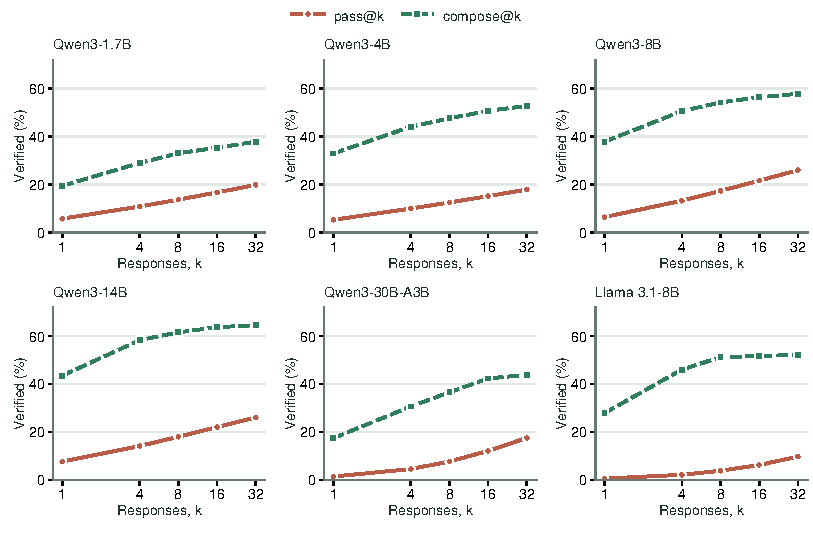
\includegraphics[width=\textwidth]{figures/base_model_probe_all.pdf}
\caption{Bare-model probe curves for all six models. Each panel compares pass@\(k\) and compose@\(k\); complete numerical results are in Table~\ref{tab:probe-complete}.}
\label{fig:appendix-probe}\label{fig:base-model-probe}\label{fig:appendix-probe-llama}
\end{figure}




Useful clauses are already recoverable at a one-response budget:
Qwen3-8B reaches 37.86\% compose@1 versus 6.43\% pass@1, and Llama 3.1-8B
reaches 27.88\% versus 0.60\%.  Additional sampling helps, but the final
budget doubling yields smaller compositional gains.  From 16 to 32
responses, compose rises from 56.37\% to 57.81\% for Qwen3-8B and from
51.68\% to 52.16\% for Llama, while pass rises from 21.63\% to 25.96\%
and from 6.25\% to 9.74\%, respectively.  These curves show diminishing
returns within the tested range; the asymptotic ceiling remains unknown.

\finishfigurewrap
\Needspace{22\baselineskip}
\subsection{Can Better Standalone Answers Make Composition Worse?}
\label{app:sft-composition-ablation}

\begin{wrapfigure}{r}{0.333333\textwidth}
\vspace{-\intextsep}
\centering
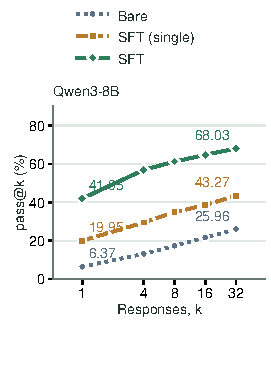
\includegraphics[width=\linewidth]{figures/sft_composition_pass.pdf}
\captionsetup{font=small}
\caption{Qwen3-8B SFT targets and pass@\(k\). Labels mark @1 and @32.}
\label{fig:sft-composition-pass}
\end{wrapfigure}




We compare Bare, SFT (single), and composed-target SFT on the same 832
programs. The two SFT datasets contain approximately equal numbers of
training examples. Single targets are independently filtered responses;
composed targets pool discoveries across responses.

SFT (single) improves pass over Bare but lowers compose at every reported
budget.  Composed-target SFT exceeds both models on both metrics: relative
to SFT (single), its compose gains are 40.70 points at \(k=1\) and 30.18
at \(k=32\), with pass gains of 22.00 and 24.76 points.  Thus better
standalone answers need not supply better compositions; supervision from
broader candidate pools improves both in this comparison.  Main-text
Figure~\ref{fig:sft-composition-compose} shows compose, and
Figure~\ref{fig:sft-composition-pass} shows pass; per-stratum data are in
Tables~\ref{tab:sft-probe-complete} and~\ref{tab:latest-sft-filter}.

\finishfigurewrap
\subsection{Reward Ablation: Should One Bad Clause Cancel All Credit?}
\label{app:ablation-definitions}



\paragraph{Reward configuration.}
The reported RL runs apply the per-response admission cap without penalizing
clauses beyond that cap, consistently with the reward definition above.

The reward variants use different correctness gates for
Equation~\ref{eq:generation-reward}.  \emph{Binary} assigns one
iff the processed response is nonempty and every clause survives Houdini.
\emph{Whole-rollout} pays the strength score
\(\operatorname{cov}(V_i)\) only when every processed clause survives,
\[
  r_i^{\mathrm{whole}}
  =\mathbf 1[V_i=
    \operatorname{Unique}(\operatorname{First}_{m_{\max}}(
      \operatorname{parts}(y_i)))]
   \frac{|R_i|}{|\mathcal N|}.
\]
\emph{Clause-decomposed} removes this all-or-nothing indicator and scores
each response by the coverage of its surviving \(V_i\).  Full (default)
adds response-level
Shapley credit: \(r_i^{\mathrm{Full}}=r_i^{\text{Clause-decomposed}}+0.3\phi_i\),
with the fixed survivor coverage game defined in
Appendix~\ref{app:formal-shapley}.
All four variants admit at most \(m_{\max}\) clauses per response and include
no separate redundancy or overflow penalty.
\begin{table}[H]
\centering
\small
\caption{Available reward ablations across backbones on all 832 programs (\%).
Full after SFT uses the main 69.23\% evaluation throughout; exploration
diagnostics are discussed in Appendix~\ref{app:full-credit-analysis}.
Qwen3-8B reward variants are reported in
Tables~\ref{tab:latest-rl-bare} and~\ref{tab:latest-rl-sft}; additional
Whole-rollout controls are in Table~\ref{tab:latest-rl-other}, and the
other-backbone Full results are in Table~\ref{tab:rl-complete}.}
\label{tab:reward-ablation}
\begin{tabular}{lrrrrrrrrrr}
\toprule
\rowcolor{algobg}
& \multicolumn{5}{c}{pass@\(k\)} & \multicolumn{5}{c}{compose@\(k\)} \\
\headercmidrules{\cmidrule(lr){2-6}\cmidrule(lr){7-11}}
\rowcolor{algobg}
Reward & 1 & 4 & 8 & 16 & 32 & 1 & 4 & 8 & 16 & 32 \\
\midrule
\multicolumn{11}{l}{\textit{Qwen3-8B, RL directly from Bare}} \\
Binary & 4.45 & 4.45 & 4.45 & 4.45 & 4.45 & 4.55 & 4.55 & 4.55 & 4.55 & 4.55 \\
Whole-rollout & 15.50 & 16.59 & 16.83 & 17.67 & 18.39 & 20.79 & 21.88 & 22.24 & 22.84 & 23.32 \\
Clause-decomposed & 9.01 & 15.87 & 18.87 & 20.31 & 21.63 & 48.80 & 57.69 & 60.70 & 63.70 & 66.35 \\
Full (default) & 2.88 & 5.41 & 7.81 & 9.62 & 11.06 & 51.80 & 60.46 & 64.18 & 68.87 & 70.67 \\
\midrule
\multicolumn{11}{l}{\textit{Qwen3-8B, RL after SFT}} \\
Binary & 8.77 & 11.30 & 13.22 & 14.30 & 15.50 & 7.09 & 10.82 & 13.34 & 14.54 & 15.99 \\
Whole-rollout & 38.82 & 45.19 & 48.68 & 50.84 & 53.73 & 43.63 & 50.12 & 53.37 & 56.01 & 58.53 \\
Clause-decomposed & 35.94 & 51.44 & 54.33 & 57.69 & 61.30 & 67.91 & 75.84 & 76.80 & 77.64 & 78.25 \\
Full (default) & 30.78 & 43.44 & 47.47 & 50.63 & 53.47 & 69.23 & 75.24 & 76.80 & 77.64 & 78.37 \\
\midrule
\multicolumn{11}{l}{\textit{Qwen3-4B, RL after SFT}} \\
Whole-rollout & 42.07 & 50.72 & 53.97 & 56.61 & 58.17 & 53.25 & 61.18 & 64.06 & 66.23 & 67.43 \\
Full (default) & 35.10 & 47.12 & 53.25 & 58.17 & 62.74 & 67.55 & 75.60 & 78.00 & 78.85 & 79.21 \\
\midrule
\multicolumn{11}{l}{\textit{Qwen3-14B, RL after SFT}} \\
Whole-rollout & 41.95 & 50.60 & 54.69 & 57.45 & 59.62 & 56.49 & 63.22 & 67.91 & 70.19 & 72.12 \\
Full (default) & 35.82 & 48.80 & 53.00 & 55.53 & 58.05 & 69.35 & 75.12 & 76.44 & 77.64 & 78.25 \\
\midrule
\multicolumn{11}{l}{\textit{Llama 3.1-8B, RL after SFT}} \\
Whole-rollout & 41.83 & 53.49 & 57.81 & 62.26 & 65.75 & 52.88 & 65.14 & 69.11 & 71.39 & 73.20 \\
Full (default) & 35.70 & 48.32 & 53.00 & 56.97 & 59.86 & 61.90 & 72.00 & 74.40 & 75.24 & 75.72 \\
\bottomrule
\end{tabular}
\end{table}

\paragraph{Preserving partial contributions improves composition.}
From Bare Qwen3-8B, Whole-rollout raises pass@1 from 6.43\% to 15.50\%
but lowers compose@32 from 57.81\% to 23.32\%.  Clause-decomposed restores
66.35\% compose@32 by crediting surviving clauses even when their response
fails.  Its advantage over Whole-rollout is 43.03 points from Bare and
19.72 points after SFT at \(k=32\), supporting clause-level credit under
both initializations.  Binary reaches only 4.55\% and 15.99\%, respectively.

Full also exceeds Whole-rollout after SFT on Qwen3-4B and Llama 3.1-8B,
by 14.30 and 9.02 points at compose@1.  These cross-backbone rows compare
the complete reward against Whole-rollout; they do not isolate the added
Shapley term.  Exploration diagnostics for Full and Clause-decomposed
are in Appendix~\ref{app:full-credit-analysis}.

\Needspace{28\baselineskip}
\subsubsection{Does Training Reward Track Verification Quality?}
\label{app:reward-training-curves}

The supplied Qwen3-8B training records cover 2 RL epochs for four rewards
under Bare and SFT initialization, giving eight complete curves.  Figure~\ref{fig:reward-training-curves}
reports the mean reward at each training step for each configuration,
as confirmed for the supplied CSV.

\begin{wrapfigure}{r}{0.666667\textwidth}
\centering
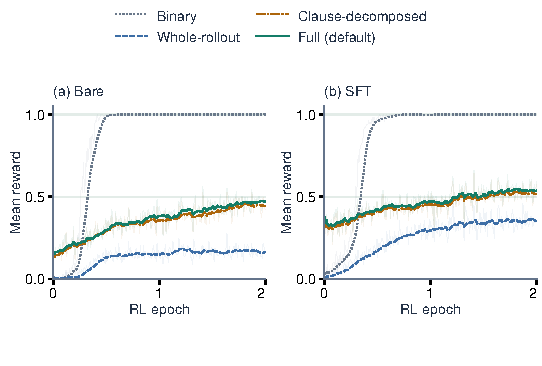
\includegraphics[width=\linewidth]{figures/reward_training_curves.pdf}
\caption{Mean training rewards under (a) Bare and (b) SFT initialization. Pale
lines show the per-step means; emphasized lines are trailing 15-step means,
using available steps at the start. Reward scales differ across objectives;
parentheses mark the default.}
\label{fig:reward-training-curves}
\end{wrapfigure}

\paragraph{Binary reward saturates without strong verification.}
In both initializations, every recorded Binary reward in the final 20 updates is
1.000.  Yet the corresponding two-epoch evaluations reach only 4.55\%
compose@32 from Bare and 15.99\% after SFT
(Table~\ref{tab:reward-ablation}).  Saturating the correctness reward
therefore does not ensure invariants strong enough to prove hidden targets.

\paragraph{Reward growth must be judged against verification.}
Full, Clause-decomposed, and Whole-rollout all end with higher rewards than
they start with under both initializations.  Their upward trajectories,
alongside Binary's saturation, show successful optimization of different
signals; the endpoint compose results determine whether that progress
produces useful invariants.  Absolute heights cannot rank the configurations:
the correctness gates differ, and Full adds weighted Shapley credit.

The CSV records per-step mean rewards. Per-group reward variance is required
to measure how often Full prevents group reward collapse. The mechanism is formalized in
Appendix~\ref{app:formal-reward-collapse}, and additional exploration diagnostics
are analyzed in Appendix~\ref{app:full-credit-analysis}.

\finishfigurewrap

\subsection{Can More Clauses Hurt Answers Yet Help Proofs?}
\label{app:clause-cap}

We vary the per-response clause cap for Bare, SFT, and SFT+RL Qwen3-8B.
Within each model, all caps reuse the same saved response pool and evaluation
settings: only the first \(c\) parsed clauses of each response are admitted
to standalone verification or pooled filtering.  This is inference-time
truncation of saved responses. The sweep is a separate evaluation; its cap-16
endpoints are not substituted for the main-result models.

\begin{table}[H]
\centering
\small
\setlength{\tabcolsep}{3pt}
\caption{Qwen3-8B clause-cap ablation (\%). Within each model, all rows reuse
 the same saved responses. Pass values use the nearest-integer projection
 of supplied rates described in Appendix~\ref{app:experimental-protocol};
 this uses the reported rates directly. Compose values retain the supplied
 results. Bold marks each column's maximum across caps.}
\label{tab:clause-cap-ablation}
\begin{tabular}{crrrrrrrrr}
\toprule
\rowcolor{algobg}
& \multicolumn{3}{c}{pass@1} & \multicolumn{3}{c}{compose@1}
& \multicolumn{3}{c}{compose@8} \\
\headercmidrules{\cmidrule(lr){2-4}\cmidrule(lr){5-7}\cmidrule(lr){8-10}}
\rowcolor{algobg}
Cap & Bare & SFT & SFT+RL & Bare & SFT & SFT+RL & Bare & SFT & SFT+RL \\
\midrule
1 & \textbf{12.14} & 19.59 & 22.84 & 11.06 & 19.23 & 22.72 & 17.67 & 35.10 & 25.48 \\
2 & 9.50 & 27.28 & 30.29 & 17.31 & 30.89 & 34.01 & 25.24 & 49.40 & 39.18 \\
4 & 8.17 & 41.47 & \textbf{45.31} & 27.76 & 45.67 & 50.48 & 40.75 & 67.07 & 57.45 \\
8 & 7.09 & \textbf{44.47} & 41.95 & 35.46 & 57.09 & 63.34 & 52.40 & 73.56 & 71.39 \\
16 & 6.61 & 42.79 & 30.89 & \textbf{39.42} & \textbf{64.90} & \textbf{69.11} & \textbf{54.21} & \textbf{76.56} & \textbf{76.32} \\
\bottomrule
\end{tabular}
\end{table}

\paragraph{The best clause budget depends on the success criterion.}
Bare pass@1 is highest at cap 1 and falls as the cap grows.  SFT and
SFT+RL instead peak at caps 8 and 4, respectively.  For SFT+RL, increasing
the cap from 4 to 16 lowers displayed pass@1 from 45.31\% to 30.89\%,
while compose@1 rises from 50.48\% to 69.11\% and compose@8 from 57.45\%
to 76.32\%.  Both compose metrics increase monotonically with the cap
for all three models in this sweep.  Additional clauses can therefore
hurt complete-response verification while expanding the candidates
available for filtering; these aggregates do not distinguish invalid
clauses from prover timeouts or other causes of standalone failure.

\paragraph{Does Better Composition Require More Distinct Clauses?}
Table~\ref{tab:clause-cap-structure} separates response length from the
number of distinct and surviving clauses across eight responses.

\begin{table}[H]
\centering
\small
\caption{Structural statistics for the same clause-cap sweep. Clauses is
 the mean admitted clause count per response; Unique@8 is the mean number
 of canonical clause keys across eight responses; Survivors@8 is the mean
 number retained after filtering their pooled union. These are mean counts.}
\label{tab:clause-cap-structure}
\begin{tabular}{llrrrrr}
\toprule
\rowcolor{algobg}
Model & Statistic & Cap 1 & Cap 2 & Cap 4 & Cap 8 & Cap 16 \\
\midrule
\multirow{3}{*}{Bare}
 & Clauses & 1.00 & 1.98 & 3.88 & 7.24 & 12.37 \\
 & Unique@8 & 2.72 & 5.50 & 11.67 & 24.30 & 41.69 \\
 & Survivors@8 & 1.42 & 2.49 & 5.37 & 11.33 & 19.91 \\
\midrule
\multirow{3}{*}{SFT}
 & Clauses & 1.00 & 2.00 & 3.96 & 7.52 & 12.73 \\
 & Unique@8 & 3.37 & 6.69 & 14.26 & 30.14 & 56.07 \\
 & Survivors@8 & 2.92 & 5.71 & 12.10 & 25.27 & 46.35 \\
\midrule
\multirow{3}{*}{SFT+RL}
 & Clauses & 1.00 & 2.00 & 4.00 & 7.98 & 14.03 \\
 & Unique@8 & 1.41 & 2.90 & 6.41 & 15.90 & 35.80 \\
 & Survivors@8 & 1.18 & 2.33 & 5.06 & 12.06 & 26.07 \\
\bottomrule
\end{tabular}
\end{table}

At cap 16, Bare and SFT admit similar numbers of clauses per response
(12.37 versus 12.73), but SFT supplies more unique clauses (56.07 versus
41.69) and more than twice as many survivors (46.35 versus 19.91).
Output length alone therefore does not explain the SFT gain.

Post-SFT RL shows a different pattern.  It admits more clauses per response
than SFT (14.03 versus 12.73), yet produces fewer unique clauses across
eight responses (35.80 versus 56.07) and fewer survivors (26.07 versus
46.35).  Nevertheless, compose@1 is 4.21 points higher, while compose@8
is nearly unchanged (76.32\% versus 76.56\%).  Thus its one-response gain
coexists with a smaller distinct candidate pool, consistent with useful
candidates becoming easier to obtain at a small sampling budget.  This
comparison does not support an increase in cross-response diversity;
clause counts alone also do not measure logical strength or necessity.

\Needspace{22\baselineskip}
\subsection{Does Negative Coverage Align with Final Verification?}

\label{app:coverage-predictiveness}

\begin{wrapfigure}{r}{0.666667\textwidth}
\vspace{-\intextsep}
\centering
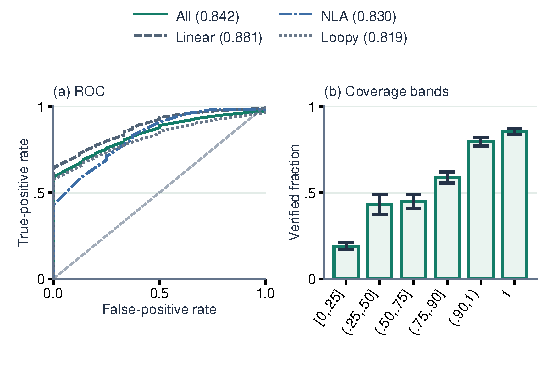
\includegraphics[width=\linewidth]{figures/negative_coverage_predictiveness.pdf}
\captionsetup{font=small}
\caption{Negative coverage on 5,711 candidate sets. (a) Macro ROC and AUROC. (b) Verification by coverage band, with Wilson 95\% intervals.}
\label{fig:coverage-predictiveness}
\end{wrapfigure}


This diagnostic evaluates negative coverage on fixed candidates.  The
population contains 5,711 candidate sets
from 691 benchmark programs with both accepted and rejected sets, including
archived target-hidden GPT-5-nano tool outputs and one verified reference
set per program.  The remaining 141 programs lack both classes for
within-program ranking.

Coverage is computed from frozen Houdini survivors and positive states using
the target-hidden program, seed 0, and a budget of 60 negative traces.  Hidden
targets supply only final Frama-C/WP labels, never scores.  AUROC is computed
within each program and macro-averaged.  Confidence intervals use 5,000
bootstrap resamples over programs.

\begin{center}
\small
\begin{tabular}{lrrr}
\toprule
\rowcolor{algobg}
Population & Programs & Candidates & Coverage AUROC \\
\midrule
Linear & 248 & 2,173 & 0.881 \\
NLA & 49 & 439 & 0.830 \\
Loopy & 394 & 3,099 & 0.819 \\
All & 691 & 5,711 & 0.842 \\
\bottomrule
\end{tabular}
\end{center}

Negative coverage achieves a macro AUROC of 0.842 (program-level bootstrap
95\% CI: \([0.826,0.858]\)), with consistent alignment across Linear, NLA,
and Loopy.  This diagnostic evaluates ranking on fixed candidates; it does not
measure the causal effect of negative-trace construction on RL training.
Coverage is an empirical diagnostic; final verification and generation
determine whether a sufficient invariant is found.

This population consists of archived tool outputs and verified references.
Training-time response groups require separate evidence of informative
within-group reward differences.



\subsection{When Does Filtering Together Beat Filtering Separately?}

\label{app:houdini-order}

We compare filtering each response before pooling (pre-filtering) with
one joint filter over the pooled clauses (post-filtering), using the same
saved Qwen3-8B response prefixes on 832 programs.  CRAFT uses the latter
order in inference and training; the operator and its theoretical properties
are defined in Appendix~\ref{app:formal-method}.

\paragraph{Joint filtering approaches the same verification rate at much lower cost.}
With the 900-second cap, post-filtering reaches 64.2\% compose@32 versus
64.4\% for pre-filtering (Table~\ref{tab:prefilt-vs-postfilt}).  The recorded
whole-workload cost is 127 versus 1,472 CPU-hours, or about 8.6\% as much.
These values are total CPU-hours for the reported 832-program evaluation
workload. The main observed advantage is avoiding repeated
filtering calls while retaining nearly the same verification rate.

\paragraph{A tight timeout can erase the benefit of a larger candidate pool.}
At a 300-second cap, post-filtering costs 113 CPU-hours but reaches only
58.7\% compose@32.  Increasing the cap to 900 seconds recovers 5.5 points
with 14 additional CPU-hours.  Thus the cost advantage depends on allowing
enough time for the larger pooled obligations; the ideal inclusion property
does not guarantee higher verification under finite prover budgets.

\begin{table}[t]
\centering
\small
\caption{Pre-filtering and post-filtering for invariant verification on the
  832-program benchmark (Qwen3-8B, saved prefixes up to 32 rollouts; compose@\(k\)
  in \%).  CPU-h is the whole-workload total.}
\label{tab:prefilt-vs-postfilt}
\begin{tabular}{ll rrrrr r}
\toprule
\rowcolor{algobg}
Method & Subset & @1 & @4 & @8 & @16 & @32 & CPU-h \\
\midrule
Post-filter (300 s)  & All    & 40.4 & 52.8 & 56.0 & 58.1 & 58.7 &  113 \\
                    & Loopy  & 43.3 & 56.9 & 60.9 & 63.1 & 63.7 &      \\
                    & Linear & 41.1 & 53.8 & 56.3 & 57.9 & 58.5 &      \\
                    & NLA    &  8.0 &  8.0 &  8.0 & 12.0 & 12.0 &      \\
\midrule
Post-filter (900 s)  & All    & 40.4 & 53.4 & 58.4 & 62.5 & 64.2 &  127 \\
                    & Loopy  & 43.3 & 57.7 & 63.3 & 68.7 & 70.2 &      \\
                    & Linear & 41.1 & 54.1 & 59.2 & 61.4 & 63.3 &      \\
                    & NLA    &  8.0 &  8.0 &  8.0 & 12.0 & 14.0 &      \\
\midrule
Pre-filter          & All    & 40.4 & 52.8 & 57.9 & 62.1 & 64.4 & 1472 \\
                    & Loopy  & 43.3 & 57.3 & 62.9 & 68.0 & 71.0 &      \\
                    & Linear & 41.1 & 53.2 & 58.5 & 61.4 & 63.0 &      \\
                    & NLA    &  8.0 &  8.0 &  8.0 & 12.0 & 12.0 &      \\
\bottomrule
\end{tabular}
\end{table}

\Needspace{22\baselineskip}
\subsection{How Does Target Visibility Change Verification and Sampling Needs?}

\label{app:target-visibility}

\begin{wrapfigure}{r}{0.666667\textwidth}
\vspace{-\intextsep}
\centering
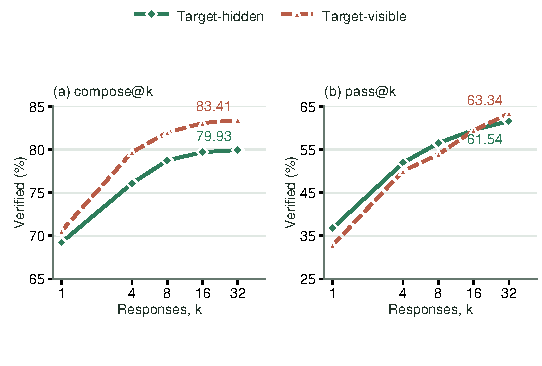
\includegraphics[width=\linewidth]{figures/target_visibility.pdf}
\captionsetup{font=small}
\caption{Target visibility for the same Qwen3-8B SFT+RL model. (a) compose@\(k\); (b) pass@\(k\). No retraining or iterative feedback.}
\label{fig:target-visibility}
\end{wrapfigure}


We expose the target assertions and postconditions during generation for
the same Qwen3-8B SFT+RL model, holding other settings and response
budgets fixed.  The model was trained with targets hidden; neither condition
adds training or iterative verifier feedback.  The hidden reference matches
Table~\ref{tab:rl-complete}.

Target visibility improves both whole-workload metrics at every tested
budget (Figure~\ref{fig:target-visibility}).  Compose gains 1.32 points at
\(k=1\) and 3.12--3.73 points at \(k\ge4\), corresponding to 11 and
26--31 additional verified programs.  Pass gains range from approximately
1.68 points at \(k=1\) to 7.21 at \(k=32\).

Visible compose@4 reaches 78.73\%, compared with 78.37\% for hidden
compose@32. Target visibility therefore reduces the sampling budget in this
evaluation. The saved-pool estimates and prefix compositions remain subject
to sampling variance (Appendix~\ref{app:limitations}).

\begin{table}[H]
\centering
\small
\caption{CRAFT with target-visible (target-vision) and target-hidden inference
using the same Qwen3-8B SFT+RL model, by benchmark stratum and sampling
budget.  Each cell reports a percentage; All / 832 is the whole-workload
result.  Visible compose rates are computed from exact success counts;
visible pass rates retain the reported one-decimal precision.  Hidden results retain the paired evaluation used in this experiment.}
\label{tab:target-visible-strata}
\begin{tabular}{lccccccccc}
\toprule
\rowcolor{algobg}
& & \multicolumn{2}{c}{Linear / 316} & \multicolumn{2}{c}{NLA / 50}
  & \multicolumn{2}{c}{Loopy / 466} & \multicolumn{2}{c}{All / 832} \\
\headercmidrules{\cmidrule(lr){3-4}\cmidrule(lr){5-6}\cmidrule(lr){7-8}\cmidrule(lr){9-10}}
\rowcolor{algobg}
Configuration & \(k\) & pass & comp & pass & comp & pass & comp & pass & comp
  \\
\midrule
\multirow{5}{*}{\shortstack[l]{CRAFT\\(target-hidden)}}
 & 1  & 32.91 & 75.00 & 2.00 & 14.00 & 32.40 & 71.24 & 30.78 & 69.23 \\
 & 4  & 46.52 & 79.75 & 4.00 & 14.00 & 45.71 & 78.76 & 43.44 & 75.24 \\
 & 8  & 50.95 & 80.70 & 4.00 & 14.00 & 49.79 & 80.90 & 47.47 & 76.80 \\
 & 16 & 54.75 & 80.70 & 4.00 & 14.00 & 53.00 & 82.40 & 50.63 & 77.64 \\
 & 32 & 57.91 & 81.33 & 4.00 & 14.00 & 55.79 & 83.26 & 53.47 & 78.37 \\
\cmidrule(l{3pt}r{3pt}){1-10}
\multirow{5}{*}{\shortstack[l]{CRAFT\\(target-vision)}}
 & 1  & 34.49 & 73.42 & 4.00 & 10.00 & 34.12 & 75.11 & 32.45 & 70.55 \\
 & 4  & 51.58 & 80.70 & 6.00 & 14.00 & 51.50 & 84.33 & 48.68 & 78.73 \\
 & 8  & 56.65 & 82.59 & 6.00 & 14.00 & 56.87 & 86.05 & 53.73 & 80.41 \\
 & 16 & 60.76 & 83.23 & 6.00 & 14.00 & 60.94 & 87.34 & 57.45 & 81.37 \\
 & 32 & 64.24 & 83.23 & 6.00 & 14.00 & 64.16 & 87.55 & 60.70 & 81.49 \\
\bottomrule
\end{tabular}
\end{table}

Table~\ref{tab:target-visible-strata} shows that the composition gains vary
by stratum.  Loopy improves at every budget, by 3.87--5.57 percentage points.
Linear improves for \(k\ge4\), but its compose@1 falls from 75.00\% to
73.42\%.  NLA compose@1 falls from 14.00\% to 10.00\%, while both conditions
reach 14.00\% for \(k\ge4\).  The target-visibility gain is concentrated in
Loopy and is absent or negative for NLA.

The results isolate the effect of target visibility without iterative
refinement.

\subsection{Does the Advantage Survive Changes in Models and Tools?}
\label{app:other-work-comparison}

We examine generator choice, verification cost with a fixed model, and
how tool interfaces and feedback conditions affect the comparison.

\subsubsection{Does the Best Standalone Model Also Compose Best?}
\label{app:rq3}
\label{app:reasoning-leakage}

Table~\ref{tab:cross-model-main} holds target hiding and reasoning-disabled
generation fixed across four API models.  Claude Sonnet-4.6 leads at
compose@1 (56.97\%), while DeepSeek V4-Flash leads at compose@8 (74.40\%).
At eight responses, GPT-5 has higher pass than DeepSeek (51.68\% versus
48.20\%) but lower compose (72.00\% versus 74.40\%).  Choosing a generator
by standalone success can therefore miss the best generator for composition.

\begin{table}[H]
\centering
\small
\caption{Complete reasoning-disabled cross-model results by benchmark stratum and
sampling budget.  Each cell reports a percentage; All / 832 is the
whole-workload result.  Rows for each model come from one archived rollout
pool of 10 responses per task.  Pass@\(k\) uses a projected estimate from the
saved response pool;
compose@\(k\) evaluates the first \(k\) saved responses.  Bold marks one maximum per metric column across all models and budgets;
ties are marked only at their first occurrence.  GPT-5-mini is excluded because it has no
reasoning-disabled setting.}
\label{tab:cross-model-main}
\begin{tabular}{lccccccccc}
\toprule
\rowcolor{algobg}
& & \multicolumn{2}{c}{Linear / 316} & \multicolumn{2}{c}{NLA / 50}
  & \multicolumn{2}{c}{Loopy / 466} & \multicolumn{2}{c}{All / 832} \\
\headercmidrules{\cmidrule(lr){3-4}\cmidrule(lr){5-6}\cmidrule(lr){7-8}\cmidrule(lr){9-10}}
\rowcolor{algobg}
Model & \(k\) & pass & comp & pass & comp & pass & comp & pass & comp \\
\midrule
\multirow{3}{*}{GPT-5-nano} & 1
  & \acc{12/316}{3.80} & \acc{110/316}{34.81} & \acc{0/50}{0.00} & \acc{11/50}{22.00} & \acc{18/466}{3.86} & \acc{161/466}{34.55} & \acc{30/832}{3.61} & \acc{282/832}{33.89} \\
 & 4
  & \acc{34/316}{10.76} & \acc{152/316}{48.10} & \acc{1/50}{2.00} & \acc{15/50}{30.00} & \acc{53/466}{11.37} & \acc{241/466}{51.72} & \acc{88/832}{10.58} & \acc{408/832}{49.04} \\
 & 8
  & \acc{50/316}{15.82} & \acc{175/316}{55.38} & \acc{2/50}{4.00} & \acc{22/50}{44.00} & \acc{82/466}{17.60} & \acc{265/466}{56.87} & \acc{134/832}{16.11} & \acc{462/832}{55.53} \\
\cmidrule(l{3pt}r{3pt}){1-10}
\multirow{3}{*}{GPT-5} & 1
  & \acc{111/316}{35.13} & \acc{165/316}{52.22} & \acc{3/50}{6.00} & \acc{18/50}{36.00} & \acc{157/466}{33.69} & \acc{244/466}{52.36} & \acc{271/832}{32.57} & \acc{427/832}{51.32} \\
 & 4
  & \acc{151/316}{47.78} & \acc{205/316}{64.87} & \acc{4/50}{8.00} & \acc{26/50}{52.00} & \acc{236/466}{50.64} & \acc{314/466}{67.38} & \acc{391/832}{47.00} & \acc{545/832}{65.50} \\
 & 8
  & \textbf{\acc{164/316}{51.90}} & \acc{222/316}{70.25} & \textbf{\acc{5/50}{10.00}} & \acc{33/50}{66.00} & \textbf{\acc{262/466}{56.22}} & \acc{344/466}{73.82} & \textbf{\acc{430/832}{51.68}} & \acc{599/832}{72.00} \\
\cmidrule(l{3pt}r{3pt}){1-10}
\multirow{3}{*}{Claude Sonnet-4.6} & 1
  & \acc{109/316}{34.49} & \acc{175/316}{55.38} & \acc{4/50}{8.00} & \acc{22/50}{44.00} & \acc{190/466}{40.77} & \acc{277/466}{59.44} & \acc{302/832}{36.30} & \acc{474/832}{56.97} \\
 & 4
  & \acc{127/316}{40.19} & \acc{199/316}{62.97} & \acc{4/50}{8.00} & \acc{26/50}{52.00} & \acc{220/466}{47.21} & \acc{309/466}{66.31} & \acc{352/832}{42.31} & \acc{534/832}{64.18} \\
 & 8
  & \acc{135/316}{42.72} & \acc{210/316}{66.46} & \acc{5/50}{10.00} & \acc{32/50}{64.00} & \acc{234/466}{50.21} & \acc{315/466}{67.60} & \acc{374/832}{44.95} & \acc{557/832}{66.95} \\
\cmidrule(l{3pt}r{3pt}){1-10}
\multirow{3}{*}{DeepSeek V4-Flash} & 1
  & \acc{91/316}{28.80} & \acc{165/316}{52.22} & \acc{3/50}{6.00} & \acc{22/50}{44.00} & \acc{140/466}{30.04} & \acc{241/466}{51.72} & \acc{234/832}{28.13} & \acc{428/832}{51.44} \\
 & 4
  & \acc{134/316}{42.41} & \acc{210/316}{66.46} & \acc{4/50}{8.00} & \acc{30/50}{60.00} & \acc{222/466}{47.64} & \acc{326/466}{69.96} & \acc{360/832}{43.27} & \acc{566/832}{68.03} \\
 & 8
  & \acc{147/316}{46.52} & \textbf{\acc{226/316}{71.52}} & \acc{4/50}{8.00} & \textbf{\acc{36/50}{72.00}} & \acc{250/466}{53.65} & \textbf{\acc{357/466}{76.61}} & \acc{401/832}{48.20} & \textbf{\acc{619/832}{74.40}} \\
\bottomrule
\end{tabular}
\end{table}

Pass displays nearest-integer projections of archived pool estimates;
compose uses saved prefixes (Appendix~\ref{app:experimental-protocol}).

\Needspace{22\baselineskip}
\subsubsection{What Verification--Cost Tradeoff Does a Fixed Model Achieve?}
\label{app:tools-comparison}

\begin{wrapfigure}{r}{0.333333\textwidth}
\vspace{-\intextsep}
\centering
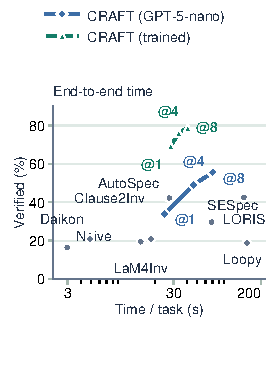
\includegraphics[width=\linewidth]{figures/tool_pareto_time.pdf}
\captionsetup{font=small}
\caption{Verification versus time under native serving setups, using each
method's full supported set. Direct GPT-5-nano results use 832 tasks except
Clause2Inv (316) and LaM4Inv (366); the dashed trained-CRAFT reference uses all
832. Daikon uses no model tokens.}
\label{fig:tool-pareto-time}
\end{wrapfigure}

On all 832 tasks, with GPT-5-nano and target hiding fixed, CRAFT compose@4
verifies 49.04\% of programs using 1,905.10 tokens per task, compared with
AutoSpec's 42.19\% and 2,216.11 tokens. AutoSpec itself pools
eight parallel proposals, so
this comparison evaluates the complete clause-processing pipelines.

SESpec iteratively repairs a running candidate and verifies 29.69\% using
22,081.61 tokens per task. CRAFT compose@1 verifies 33.89\% with 1,136.82
tokens. LORIS verifies 42.55\% but uses 47,816.27 tokens per task; LaM4Inv
verifies 19.40\% using 1,470.80 tokens on its supported 366 tasks. This comparison
supports clause reuse under limited target feedback; the native pipelines
also differ in extraction and repair, so it does not isolate orchestration
as the only cause.

Figure~\ref{fig:tool-pareto-time} adds measured end-to-end time to the token
comparison.  Table~\ref{tab:trained-cost-run} reports the selected trained
model separately on all 832 tasks: it reaches 69.23\%, 75.24\%, and 76.80\% at compose@1,
@4, and @8 in 28.22, 33.53, and 40.90 seconds per task.  At @4 and @8 it
uses less recorded time than the corresponding GPT-5-nano CRAFT runs
(46.40 and 69.99 seconds), but it is not part of the fixed-model direct
comparison.  Verification rates follow the
selected Qwen3-8B + SFT + RL result; costs are the recorded local cost-run
measurements. Times reflect each method's native serving setup;
GPT-5-nano CRAFT combines archived request
latency with measured filtering and final verification.

Table~\ref{tab:tools-complete} reports all results; the parameter settings
are in Table~\ref{tab:tool-sampling-parameters}.  Daikon incurs verification
time but uses no model tokens.  Tool-specific applicability and extraction
limitations are discussed immediately below the tables.

\finishfigurewrap
\begin{table}[H]
\centering
\small
\caption{Verification and inference cost of the selected trained CRAFT model.
Verification rates are from Qwen3-8B + SFT + RL; token and time values are
the recorded local cost-run measurements.}
\label{tab:trained-cost-run}
\begin{tabular}{llrrrrrr}
\toprule
\rowcolor{algobg}
Method & Reason. & Linear & NLA & Loopy & All & Tokens/task & Time/task \\
\midrule
\sam{} (compose@1) & none & \acc{237}{75.00\%} & \acc{7}{14.00\%}
  & \acc{332}{71.24\%} & \acc{576}{69.23\%} & 1,348.23 & 28.22\,s \\
\sam{} (compose@4) & none & \acc{252}{79.75\%} & \acc{7}{14.00\%}
  & \acc{367}{78.76\%} & \acc{626}{75.24\%} & 2,053.71 & 33.53\,s \\
\sam{} (compose@8) & none & \acc{255}{80.70\%} & \acc{7}{14.00\%}
  & \acc{377}{80.90\%} & \acc{639}{76.80\%} & 2,993.44 & 40.90\,s \\
\bottomrule
\end{tabular}
\end{table}

\begin{table}[H]
\centering
\small
\caption{Complete reasoning-disabled, target-hidden comparison underlying
Figure~\ref{fig:tool-pareto}. Supported Total uses each method's full supported
set: 832 tasks where applicable, 366 for LaM4Inv, and 316 for Clause2Inv.
An em dash denotes a category that was not evaluated and is not counted as
failed; the reasons are summarized below the table.
The CRAFT compose rows are prefix compositions of the same archived
ten-rollout pool.}
\label{tab:tools-complete}
\begin{tabular}{llrrrrrr}
\toprule
\rowcolor{algobg}
Method & Reason. & Linear & NLA & Loopy & Supported Total & Tokens/task & Time/task \\
\midrule
AutoSpec & none & \acc{151}{47.78\%} & \acc{3}{6.00\%} & \acc{197}{42.27\%}
  & \acc{351/832}{42.19\%}
  & 2,216.11 & 27.34\,s \\
SESpec & none & \acc{91}{28.80\%} & \acc{2}{4.00\%} & \acc{154}{33.05\%}
  & \acc{247/832}{29.69\%}
  & 22,081.61 & 68.50\,s \\
Clause2Inv & none & \acc{66}{20.89\%} & --- & ---
  & \acc{66/316}{20.89\%}
  & 1,461.80 & 18.37\,s \\
LORIS & none & \acc{133}{42.09\%} & \acc{11}{22.00\%} & \acc{210}{45.06\%}
  & \acc{354/832}{42.55\%}
  & 47,816.27 & 138.17\,s \\
LaM4Inv & none & \acc{70}{22.15\%} & \acc{1}{2.00\%} & ---
  & \acc{71/366}{19.40\%}
  & 1,470.80 & 14.70\,s \\
Daikon & --- & \acc{73}{23.10\%} & \acc{0}{0.00\%} & \acc{101}{21.67\%}
  & \acc{174/832}{20.91\%}
  & 0 & 4.89\,s \\
Loopy & none & \acc{64}{20.25\%} & \acc{0}{0.00\%} & \acc{92}{19.74\%}
  & \acc{156/832}{18.75\%}
  & 14,513.37 & 147.16\,s \\
\midrule
Naive & none & \acc{48}{15.19\%} & \acc{1}{2.00\%} & \acc{88}{18.88\%}
  & \acc{137/832}{16.47\%}
  & 225.95 & 2.98\,s \\
\sam{} (pass@1) & none & \acc{8/316}{2.53\%} & \acc{0/50}{0.00\%} & \acc{22/466}{4.72\%}
  & \acc{30/832}{3.61\%}
  & 1,136.82 & 7.86\,s \\
\sam{} (compose@1) & none & \acc{110}{34.81\%} & \acc{11}{22.00\%} & \acc{161}{34.55\%}
  & \acc{282/832}{33.89\%}
  & 1,136.82 & 24.52\,s \\
\sam{} (compose@4) & none & \acc{152}{48.10\%} & \acc{15}{30.00\%} & \acc{241}{51.72\%}
  & \acc{408/832}{49.04\%}
  & 1,905.10 & 46.40\,s \\
\sam{} (compose@8) & none & \acc{175}{55.38\%} & \acc{22}{44.00\%} & \acc{265}{56.87\%}
  & \acc{462/832}{55.53\%}
  & 2,929.47 & 69.99\,s \\
\bottomrule
\end{tabular}
\end{table}

\begin{table}[H]
\centering
\caption{Sampling parameters used in the reasoning-disabled target-hidden tool comparison.}
\label{tab:tool-sampling-parameters}
\begin{tabular}{lllll}
\toprule
\rowcolor{algobg}
Method & Sampling budget / task & Temperature / top-\(p\) & Completion cap & Reasoning \\
\midrule
AutoSpec & 8 & 1.0 / 1.0 & 8,192 & none \\
SESpec & 1 initial + up to 3 refinements per phase & 1.0 / 1.0 & 8,192 & none \\
Clause2Inv & adaptive; 1 per call & 1.0 / 1.0 & 8,192 & none \\
LORIS & 1 initial + adaptive local-proof repairs & 1.0 / 1.0 & 8,192 & none \\
LaM4Inv & 5 initial + adaptive VC repairs & 1.0 / 1.0 & 8,192 & none \\
Daikon & no model call & -- & -- & -- \\
Naive & 1 & 1.0 / 1.0 & 8,192 & none \\
\sam{} & 1, 4, or 8 & 1.0 / 1.0 & 8,192 & none \\
Loopy & 15 initial + up to 7 repairs & 0.7 / 1.0 & 8,192 & none \\
\bottomrule
\end{tabular}
\end{table}

For the direct-comparison rows, token and time means use each method's full
supported set. Verification denominators likewise retain every supported task.
Token means use exact provider usage where available. AutoSpec's token mean is
over its 674 exact-usage tasks; 154 legacy rows with tokenizer estimates and
four rows with unavailable usage are excluded. AutoSpec issues one request
with (n=8), so provider usage counts the prompt once and aggregates
completion tokens across all eight choices. Four LORIS runs that reached the
native time limit have unavailable final usage records and remain failures in
the verification denominator. The trained-model table is a separate all-832
reference.

For matched comparisons, CRAFT compose@4 reaches 49.04\% on the 832 tasks
used by LORIS (versus 42.55\%), 45.63\% on the 366 tasks used by LaM4Inv
(versus 19.40\%), and 48.10\% on the 316 Linear tasks used by Clause2Inv
(versus 20.89\%).

\subsubsection{Which Interface and Feedback Conditions Explain Tool Differences?}

\paragraph{Applicability affects the benchmark denominator.}
Clause2Inv normally derives false-state counterexamples from the
postcondition, which is unavailable under target hiding.  LaM4Inv likewise
uses postcondition verification conditions in its native refinement loop, and
LORIS asks the model to repair reasoning for failed target-facing verification
conditions~\citep{cao2025clause2inv,wu2024lam4inv,li2026loris}.  For the direct
comparison, we remove target/postcondition feedback from all three systems,
retain only target-independent initiation and preservation feedback, fix
GPT-5-nano with reasoning disabled, and apply the same restored-target final
judge.  Results therefore characterize uniform target-hidden adaptations,
not the systems' native target-visible configurations.

The released Clause2Inv VC pipeline has no compatible native interface for
NLA or Loopy, so neither category is evaluated. LaM4Inv's required CFG/SMT
intermediate artifacts are unavailable for Loopy, so it is not evaluated
there either. LORIS has no such restriction and is evaluated on all 466 Loopy
tasks. None of the omitted Clause2Inv/LaM4Inv categories is counted as failed.

\paragraph{Why Quokka is not added to the experimental plot.}
Quokka (formerly introduced with the InvBench benchmark) evaluates 866
SV-COMP instances, fine-tunes on 3,589 separate training instances, and
directly tests whether a generated invariant helps prove the visible target
assertion~\citep{wei2025invbench}.  Its benchmark scope, supervised data,
target visibility, backend, and acceleration-oriented outcome therefore do
not match the target-hidden, common-Frama-C evaluation here.  We discuss it as
related evidence, but do not treat its published number as a directly
comparable experimental point.

\paragraph{Extraction can prevent generated annotations from reaching verification.}
Loopy's initial responses contain invariant annotations in 98.8\% of cases,
but its native extractor passes only 1.75\% of initial responses to Houdini.
These interface measurements help explain why generating annotations does
not necessarily produce verifier-consumable candidates.

\paragraph{Configuration is part of the comparison.}
The direct rows deliberately hold the generator, disabled-reasoning setting,
target boundary, supported tasks, and final verifier fixed.  Results from
native target-visible workflows or different reasoning settings are therefore
reported only as contextual evidence, not mixed into the supported-set rates.

\subsection{Shapley Analysis: Does Group Credit Help Exploration?}
\label{app:full-credit-analysis}

We compare Full with Clause-decomposed on Qwen3-8B to examine when added
group credit helps from Bare versus SFT after 2 RL epochs.

At equal coverage, Full gives more credit to traces rejected by fewer
responses, encouraging complementary effective coverage.  The allocation
and its Shapley equivalence are defined in Appendix~\ref{app:formal-shapley}.

Table~\ref{tab:full-credit-comparison} compares Clause-decomposed and Full on
Qwen3-8B after 2 RL epochs, with target-hidden negative-trace construction and 9,024
training programs. Full after SFT uses the main evaluation at 69.23\%
compose@1, consistently with Tables~\ref{tab:rl-complete}
and~\ref{tab:reward-ablation}.

\begin{table}[H]
\centering
\small
\caption{Clause-decomposed versus Full for Qwen3-8B after 2 RL epochs (\%). Full is the default reward; the post-SFT Full row uses the main evaluation. Bold marks the better reward within each initialization and metric column, including ties.}
\label{tab:full-credit-comparison}
\begin{tabular}{lrrrrrrrrrr}
\toprule
\rowcolor{algobg}
& \multicolumn{5}{c}{pass@\(k\)} & \multicolumn{5}{c}{compose@\(k\)} \\
\headercmidrules{\cmidrule(lr){2-6}\cmidrule(lr){7-11}}
\rowcolor{algobg}
Reward & 1 & 4 & 8 & 16 & 32 & 1 & 4 & 8 & 16 & 32 \\
\midrule
\multicolumn{11}{l}{\textit{RL from Bare}} \\
Clause-decomposed & \textbf{9.01} & \textbf{15.87} & \textbf{18.87} & \textbf{20.31} & \textbf{21.63} & 48.80 & 57.69 & 60.70 & 63.70 & 66.35 \\
Full (default) & 2.88 & 5.41 & 7.81 & 9.62 & 11.06 & \textbf{51.80} & \textbf{60.46} & \textbf{64.18} & \textbf{68.87} & \textbf{70.67} \\
\midrule
\multicolumn{11}{l}{\textit{RL after SFT}} \\
Clause-decomposed & \textbf{35.94} & \textbf{51.44} & \textbf{54.33} & \textbf{57.69} & \textbf{61.30} & 67.91 & \textbf{75.84} & \textbf{76.80} & \textbf{77.64} & 78.25 \\
Full (default) & 30.78 & 43.44 & 47.47 & 50.63 & 53.47 & \textbf{69.23} & 75.24 & \textbf{76.80} & \textbf{77.64} & \textbf{78.37} \\
\bottomrule
\end{tabular}
\end{table}

\paragraph{From Bare, Full improves composition throughout the tested budgets.}
Full improves compose by 2.77--5.17 points across the tested budgets,
including 48.80\% to 51.80\% at \(k=1\) and 66.35\% to 70.67\% at
\(k=32\).  Its advantage remains substantial at the largest measured
budget, while pass decreases by 6.13--11.06 points: better composition
can accompany less successful complete responses.

\paragraph{After SFT, the added benefit is small.}
Full changes compose by \(-0.60\) to \(+1.32\) points: 67.91\% to
69.23\% at \(k=1\), and 78.25\% to 78.37\% at \(k=32\). It is lower
at \(k=4\) and tied at \(k=8\) and \(k=16\). Pass decreases by
5.17--8.05 points. Thus the added composition benefit after SFT is small
and concentrated at the one-response budget. Composed-target SFT already
supplies much of the coverage encouraged by group credit.

\paragraph{Does Full retain more policy entropy?}

The supplied training diagnostics compare Full and Clause-decomposed over
2 RL epochs. Table~\ref{tab:shapley-entropy} reports an early reference
measurement and the end-of-training value. Retention is computed from the
displayed entropy values; these are policy statistics.

\begin{table}[H]
\centering
\small
\caption{Policy entropy under the two rewards over 2 RL epochs. Retention
is final entropy divided by the early reference value. Bold marks the
higher final entropy and retention within each initialization.}
\label{tab:shapley-entropy}
\begin{tabular}{llrrr}
\toprule
\rowcolor{algobg}
Initialization & Reward & Early entropy & Final entropy & Retention (\%) \\
\midrule
\multirow{2}{*}{SFT} & Full (default) & 0.3195 & \textbf{0.1842} & \textbf{57.7} \\
 & Clause-decomposed & 0.3233 & 0.1323 & 40.9 \\
\midrule
\multirow{2}{*}{Bare} & Full (default) & 0.0588 & \textbf{0.0130} & \textbf{22.1} \\
 & Clause-decomposed & 0.0773 & 0.0120 & 15.5 \\
\bottomrule
\end{tabular}
\end{table}

Full retains more policy entropy under both initializations. The absolute
final-entropy difference is larger after SFT (0.1842 versus 0.1323) than
from Bare (0.0130 versus 0.0120); Bare also starts from unequal reference
entropies. These observations suggest that Full slows entropy loss during
training.

\paragraph{Reward dispersion and policy entropy.}
The training summary reports a batch mean-to-maximum reward ratio
0.01--0.06 lower for Full than for Clause-decomposed.

Full improves compose@\(k\) from Bare and retains higher policy entropy than
Clause-decomposed. The Shapley mechanism and its limits are formalized in
Appendix~\ref{app:formal-reward-collapse}.

\endgroup

\section{Detailed Limitations}
\label{app:limitations}

\paragraph{Sampling variance and metric aggregation.}
Archived pass@\(k\) estimates standalone success over subsets of a saved
response pool; compose@\(k\) evaluates one prefix. The displayed
pass values project reported estimates to integer counts; they do not
recover observed verdicts or ensure additive stratum counts.  Sharing the
nominal budget does not pair the individual responses used in the two
aggregates or equalize their variance.  Reordering a fixed pool leaves its
pass estimate unchanged but can alter compose.  Small differences and
apparent saturation can therefore reflect the sampled pool and prefix;
nested budgets also make curve points correlated.  Direct-count results
retain the supplied run's sampling variability.  These measurements do not
establish statistical significance or an asymptotic ceiling.  Repeating
generation and evaluating both metrics on the same sampled subsets would
permit uncertainty estimates for paired differences.

\paragraph{Program scope.}
Our implementation targets numerical programs with one scalar-integer loop.
The evaluation excludes nested loops and invariants over arrays, heaps, or
recursively defined predicates. The negative-trace construction probes scalar
arithmetic relations and exit boundaries~\citep{liu2024towards}.

\paragraph{Conditional reachability of negative traces.}
Nondeterminism, truncated or sparsely recorded traces, and unrecorded state
affecting execution can prevent cleaning from establishing unreachability.
The sampler uses sparse recording for long runs and calls no general
unreachability solver.  Coverage is therefore an empirical strength signal;
\textsf{unknown} evaluations count as non-rejection and may underestimate it.
Final soundness is established independently by Frama-C/WP.

\paragraph{Inference engine.}
Local base and trained models are served with vLLM.  In preliminary
comparisons under nominally matched decoding settings, these models had
lower verification rates with vLLM than with the other evaluated backends.
API models retain their provider serving interfaces and chat templates.  The
reported decoding and reasoning controls are applied to each backend.

\paragraph{Verifier and specification language.}
Our filtering and all final judgments use Frama-C/WP, and candidates use ACSL.
Parser behavior, generated obligations, prover integration, and syntax affect
which clauses survive.  The reported results characterize this verifier,
specification language, and source language.

\paragraph{Finite candidate-pool approximation.}
Before Houdini, the pipeline implementation applies a lightweight AST-based
filter to parse, normalize, and deduplicate candidate clauses.  Clauses outside
its supported ACSL subset are omitted.  Each response contributes at most
\(m_{\max}\) clauses before global pooling; later clauses in that response are
truncated, while no separate cap is applied to the pooled union.

\paragraph{Feedback regime.}
The evaluation covers target-independent training and finite-budget
composition without iterative verifier-feedback optimization.  In pilot runs,
models reached inductive but weak invariants: the invariants passed induction,
while the hidden goals left the verifier without a target-directed signal for
the missing behavioral strength.  The marginal gain from refinement decreased
as the initial rollout pool grew.

\paragraph{Training variance.}
We did not repeat training and inference multiple times for every experimental
configuration.
